\documentclass[twoside]{book}

% Packages required by doxygen
\usepackage{fixltx2e}
\usepackage{calc}
\usepackage{doxygen}
\usepackage[export]{adjustbox} % also loads graphicx
\usepackage{graphicx}
\usepackage[utf8]{inputenc}
\usepackage{makeidx}
\usepackage{multicol}
\usepackage{multirow}
\PassOptionsToPackage{warn}{textcomp}
\usepackage{textcomp}
\usepackage[nointegrals]{wasysym}
\usepackage[table]{xcolor}

% Font selection
\usepackage[T1]{fontenc}
\usepackage[scaled=.90]{helvet}
\usepackage{courier}
\usepackage{amssymb}
\usepackage{sectsty}
\renewcommand{\familydefault}{\sfdefault}
\allsectionsfont{%
  \fontseries{bc}\selectfont%
  \color{darkgray}%
}
\renewcommand{\DoxyLabelFont}{%
  \fontseries{bc}\selectfont%
  \color{darkgray}%
}
\newcommand{\+}{\discretionary{\mbox{\scriptsize$\hookleftarrow$}}{}{}}

% Page & text layout
\usepackage{geometry}
\geometry{%
  a4paper,%
  top=2.5cm,%
  bottom=2.5cm,%
  left=2.5cm,%
  right=2.5cm%
}
\tolerance=750
\hfuzz=15pt
\hbadness=750
\setlength{\emergencystretch}{15pt}
\setlength{\parindent}{0cm}
\setlength{\parskip}{3ex plus 2ex minus 2ex}
\makeatletter
\renewcommand{\paragraph}{%
  \@startsection{paragraph}{4}{0ex}{-1.0ex}{1.0ex}{%
    \normalfont\normalsize\bfseries\SS@parafont%
  }%
}
\renewcommand{\subparagraph}{%
  \@startsection{subparagraph}{5}{0ex}{-1.0ex}{1.0ex}{%
    \normalfont\normalsize\bfseries\SS@subparafont%
  }%
}
\makeatother

% Headers & footers
\usepackage{fancyhdr}
\pagestyle{fancyplain}
\fancyhead[LE]{\fancyplain{}{\bfseries\thepage}}
\fancyhead[CE]{\fancyplain{}{}}
\fancyhead[RE]{\fancyplain{}{\bfseries\leftmark}}
\fancyhead[LO]{\fancyplain{}{\bfseries\rightmark}}
\fancyhead[CO]{\fancyplain{}{}}
\fancyhead[RO]{\fancyplain{}{\bfseries\thepage}}
\fancyfoot[LE]{\fancyplain{}{}}
\fancyfoot[CE]{\fancyplain{}{}}
\fancyfoot[RE]{\fancyplain{}{\bfseries\scriptsize Generated by Doxygen }}
\fancyfoot[LO]{\fancyplain{}{\bfseries\scriptsize Generated by Doxygen }}
\fancyfoot[CO]{\fancyplain{}{}}
\fancyfoot[RO]{\fancyplain{}{}}
\renewcommand{\footrulewidth}{0.4pt}
\renewcommand{\chaptermark}[1]{%
  \markboth{#1}{}%
}
\renewcommand{\sectionmark}[1]{%
  \markright{\thesection\ #1}%
}

% Indices & bibliography
\usepackage{natbib}
\usepackage[titles]{tocloft}
\setcounter{tocdepth}{3}
\setcounter{secnumdepth}{5}
\makeindex

% Custom commands
\newcommand{\clearemptydoublepage}{%
  \newpage{\pagestyle{empty}\cleardoublepage}%
}

\usepackage{caption}
\captionsetup{labelsep=space,justification=centering,font={bf},singlelinecheck=off,skip=4pt,position=top}

%===== C O N T E N T S =====

\begin{document}

% Titlepage & ToC
\pagenumbering{alph}
\begin{titlepage}
\vspace*{7cm}
\begin{center}%
{\Large Co\+Chat }\\
\vspace*{1cm}
{\large Generated by Doxygen 1.8.13}\\
\end{center}
\end{titlepage}
\clearemptydoublepage
\pagenumbering{roman}
\tableofcontents
\clearemptydoublepage
\pagenumbering{arabic}

%--- Begin generated contents ---
\chapter{Readme}
\label{md___users_antonukhanov__p2_p-_chat__client__readme}
\input{md___users_antonukhanov__p2_p-_chat__client__readme}
\chapter{Namespace Index}
\section{Namespace List}
Here is a list of all namespaces with brief descriptions\+:\begin{DoxyCompactList}
\item\contentsline{section}{\hyperlink{namespace_ui}{Ui} }{\pageref{namespace_ui}}{}
\end{DoxyCompactList}

\chapter{Hierarchical Index}
\section{Class Hierarchy}
This inheritance list is sorted roughly, but not completely, alphabetically\+:\begin{DoxyCompactList}
\item \contentsline{section}{Byte\+Block}{\pageref{class_byte_block}}{}
\item \contentsline{section}{C\+F\+B\+\_\+\+Mode$<$ Cipher\+Type $>$}{\pageref{class_c_f_b___mode}}{}
\item \contentsline{section}{Kuznyechik}{\pageref{class_kuznyechik}}{}
\item \contentsline{section}{Peer}{\pageref{class_peer}}{}
\item Q\+Dialog\begin{DoxyCompactList}
\item \contentsline{section}{issuecreator}{\pageref{classissuecreator}}{}
\end{DoxyCompactList}
\item Q\+Main\+Window\begin{DoxyCompactList}
\item \contentsline{section}{Client\+Window}{\pageref{class_client_window}}{}
\end{DoxyCompactList}
\end{DoxyCompactList}

\chapter{Class Index}
\section{Class List}
Here are the classes, structs, unions and interfaces with brief descriptions\+:\begin{DoxyCompactList}
\item\contentsline{section}{\textbf{ Byte\+Block} \\*Класс из библиотеки-\/реализации алгоритма \char`\"{}Кузнечик\char`\"{}. Ссылка на документацию -\/ в источниках }{\pageref{class_byte_block}}{}
\item\contentsline{section}{\textbf{ C\+F\+B\+\_\+\+Mode$<$ Cipher\+Type $>$} \\*Класс из библиотеки-\/реализации алгоритма \char`\"{}Кузнечик\char`\"{}. Ссылка на документацию -\/ в источниках }{\pageref{class_c_f_b___mode}}{}
\item\contentsline{section}{\textbf{ Client\+Window} \\*Класс, предоставляющий интерфейc пользователя }{\pageref{class_client_window}}{}
\item\contentsline{section}{\textbf{ issuecreator} \\*Класс, предоставляющий интерфейc для создания Github Issues }{\pageref{classissuecreator}}{}
\item\contentsline{section}{\textbf{ Kuznyechik} \\*Класс из библиотеки-\/реализации алгоритма \char`\"{}Кузнечик\char`\"{}. Ссылка на документацию -\/ в источниках }{\pageref{class_kuznyechik}}{}
\item\contentsline{section}{\textbf{ Peer} \\*Класс, предоставляющий интерфейс для хранения данных о каждом \char`\"{}знакомом\char`\"{} пире }{\pageref{class_peer}}{}
\end{DoxyCompactList}

\chapter{File Index}
\section{File List}
Here is a list of all files with brief descriptions\+:\begin{DoxyCompactList}
\item\contentsline{section}{/\+Users/antonukhanov/\+P2\+P-\/\+Chat/\+Client/\textbf{ clientwindow.\+cpp} }{\pageref{clientwindow_8cpp}}{}
\item\contentsline{section}{/\+Users/antonukhanov/\+P2\+P-\/\+Chat/\+Client/\textbf{ clientwindow.\+h} }{\pageref{clientwindow_8h}}{}
\item\contentsline{section}{/\+Users/antonukhanov/\+P2\+P-\/\+Chat/\+Client/\textbf{ issuecreator.\+cpp} }{\pageref{issuecreator_8cpp}}{}
\item\contentsline{section}{/\+Users/antonukhanov/\+P2\+P-\/\+Chat/\+Client/\textbf{ issuecreator.\+h} }{\pageref{issuecreator_8h}}{}
\item\contentsline{section}{/\+Users/antonukhanov/\+P2\+P-\/\+Chat/\+Client/\textbf{ Kuznyechik.\+cpp} }{\pageref{_kuznyechik_8cpp}}{}
\item\contentsline{section}{/\+Users/antonukhanov/\+P2\+P-\/\+Chat/\+Client/\textbf{ Kuznyechik.\+hpp} }{\pageref{_kuznyechik_8hpp}}{}
\item\contentsline{section}{/\+Users/antonukhanov/\+P2\+P-\/\+Chat/\+Client/\textbf{ main.\+cpp} }{\pageref{main_8cpp}}{}
\item\contentsline{section}{/\+Users/antonukhanov/\+P2\+P-\/\+Chat/\+Client/\textbf{ mycrypto.\+cpp} }{\pageref{mycrypto_8cpp}}{}
\item\contentsline{section}{/\+Users/antonukhanov/\+P2\+P-\/\+Chat/\+Client/\textbf{ mycrypto.\+hpp} }{\pageref{mycrypto_8hpp}}{}
\item\contentsline{section}{/\+Users/antonukhanov/\+P2\+P-\/\+Chat/\+Client/\textbf{ peer.\+cpp} }{\pageref{peer_8cpp}}{}
\item\contentsline{section}{/\+Users/antonukhanov/\+P2\+P-\/\+Chat/\+Client/\textbf{ peer.\+h} }{\pageref{peer_8h}}{}
\end{DoxyCompactList}

\chapter{Namespace Documentation}
\hypertarget{namespace_ui}{}\section{Ui Namespace Reference}
\label{namespace_ui}\index{Ui@{Ui}}

\chapter{Class Documentation}
\hypertarget{class_byte_block}{}\section{Byte\+Block Class Reference}
\label{class_byte_block}\index{Byte\+Block@{Byte\+Block}}


Класс из библиотеки-\/реализации алгоритма \char`\"{}Кузнечик\char`\"{}. Ссылка на документацию -\/ в источниках.  




{\ttfamily \#include $<$mycrypto.\+hpp$>$}

\subsection*{Public Member Functions}
\begin{DoxyCompactItemize}
\item 
\hyperlink{class_byte_block_a39169d96104d9cb1016065e19c2b032e}{Byte\+Block} (size\+\_\+t size\+\_\+=0, \hyperlink{mycrypto_8hpp_a4ae1dab0fb4b072a66584546209e7d58}{B\+Y\+TE} init\+\_\+value=0)
\item 
\hyperlink{class_byte_block_aac1e3e7f8030c711a76aec7f716ce6ef}{Byte\+Block} (\hyperlink{mycrypto_8hpp_a4ae1dab0fb4b072a66584546209e7d58}{B\+Y\+TE} $\ast$p\+Blocks\+\_\+, size\+\_\+t size\+\_\+)
\item 
\hyperlink{class_byte_block_a1609a4a3919796383a94df4471e02478}{Byte\+Block} (\hyperlink{class_byte_block}{Byte\+Block} \&\&rhs)
\item 
\hyperlink{class_byte_block_ae34629ddad3e2185596f6fb346fb0dd8}{$\sim$\+Byte\+Block} ()
\item 
void \hyperlink{class_byte_block_af34224909c38e21d94d5c869599516ff}{operator=} (\hyperlink{class_byte_block}{Byte\+Block} \&\&rhs)
\item 
\hyperlink{mycrypto_8hpp_a4ae1dab0fb4b072a66584546209e7d58}{B\+Y\+TE} $\ast$ \hyperlink{class_byte_block_af61ceea6259a82189d1576f16931a9bf}{byte\+\_\+ptr} ()
\item 
const \hyperlink{mycrypto_8hpp_a4ae1dab0fb4b072a66584546209e7d58}{B\+Y\+TE} $\ast$ \hyperlink{class_byte_block_ad1cca46563041dfa94469213e71eeab6}{byte\+\_\+ptr} () const
\item 
\hyperlink{mycrypto_8hpp_a4ae1dab0fb4b072a66584546209e7d58}{B\+Y\+TE} \& \hyperlink{class_byte_block_a512ce89c574508343ed1c80c7422ae71}{operator\mbox{[}$\,$\mbox{]}} (size\+\_\+t index)
\item 
\hyperlink{mycrypto_8hpp_a4ae1dab0fb4b072a66584546209e7d58}{B\+Y\+TE} \hyperlink{class_byte_block_a1188eeaf7da2316bdca468ea91727cd2}{operator\mbox{[}$\,$\mbox{]}} (size\+\_\+t index) const
\item 
bool \hyperlink{class_byte_block_a08193b9eb12da9889420f95bee6ce610}{operator==} (const \hyperlink{class_byte_block}{Byte\+Block} \&lhs) const
\item 
bool \hyperlink{class_byte_block_a083e6c9d3ec3e39d79953eb48551d0cf}{operator!=} (const \hyperlink{class_byte_block}{Byte\+Block} \&lhs) const
\item 
void \hyperlink{class_byte_block_aba0c3bafa18238bb269ec40962baa3c1}{reset} (const \hyperlink{mycrypto_8hpp_a4ae1dab0fb4b072a66584546209e7d58}{B\+Y\+TE} $\ast$p\+Blocks\+\_\+, size\+\_\+t size\+\_\+)
\item 
size\+\_\+t \hyperlink{class_byte_block_a160a348384c35cd7beae4e123b74bf18}{size} () const
\item 
\hyperlink{class_byte_block}{Byte\+Block} \hyperlink{class_byte_block_a67954bc5c1f34b2ab865bacb777c9f37}{deep\+\_\+copy} () const
\item 
\hyperlink{class_byte_block}{Byte\+Block} \hyperlink{class_byte_block_ad60eb576a039f436736d35e3a6d09131}{operator()} (size\+\_\+t begin, size\+\_\+t length) const
\end{DoxyCompactItemize}
\subsection*{Private Attributes}
\begin{DoxyCompactItemize}
\item 
\hyperlink{mycrypto_8hpp_a4ae1dab0fb4b072a66584546209e7d58}{B\+Y\+TE} $\ast$ \hyperlink{class_byte_block_a9cc668dbb2b3562e1b72b2265f3bc077}{p\+Blocks}
\item 
size\+\_\+t \hyperlink{class_byte_block_a96ef9896e7d4a252485bbac909c7cb76}{amount\+\_\+of\+\_\+bytes}
\end{DoxyCompactItemize}
\subsection*{Friends}
\begin{DoxyCompactItemize}
\item 
void \hyperlink{class_byte_block_aff71aa0d084ae3b604be05fa66e1d4cd}{swap} (\hyperlink{class_byte_block}{Byte\+Block} \&lhs, \hyperlink{class_byte_block}{Byte\+Block} \&rhs)
\end{DoxyCompactItemize}


\subsection{Detailed Description}
Класс из библиотеки-\/реализации алгоритма \char`\"{}Кузнечик\char`\"{}. Ссылка на документацию -\/ в источниках. 

\subsection{Constructor \& Destructor Documentation}
\mbox{\Hypertarget{class_byte_block_a39169d96104d9cb1016065e19c2b032e}\label{class_byte_block_a39169d96104d9cb1016065e19c2b032e}} 
\index{Byte\+Block@{Byte\+Block}!Byte\+Block@{Byte\+Block}}
\index{Byte\+Block@{Byte\+Block}!Byte\+Block@{Byte\+Block}}
\subsubsection{\texorpdfstring{Byte\+Block()}{ByteBlock()}\hspace{0.1cm}{\footnotesize\ttfamily [1/3]}}
{\footnotesize\ttfamily Byte\+Block\+::\+Byte\+Block (\begin{DoxyParamCaption}\item[{size\+\_\+t}]{size\+\_\+ = {\ttfamily 0},  }\item[{\hyperlink{mycrypto_8hpp_a4ae1dab0fb4b072a66584546209e7d58}{B\+Y\+TE}}]{init\+\_\+value = {\ttfamily 0} }\end{DoxyParamCaption})}

\mbox{\Hypertarget{class_byte_block_aac1e3e7f8030c711a76aec7f716ce6ef}\label{class_byte_block_aac1e3e7f8030c711a76aec7f716ce6ef}} 
\index{Byte\+Block@{Byte\+Block}!Byte\+Block@{Byte\+Block}}
\index{Byte\+Block@{Byte\+Block}!Byte\+Block@{Byte\+Block}}
\subsubsection{\texorpdfstring{Byte\+Block()}{ByteBlock()}\hspace{0.1cm}{\footnotesize\ttfamily [2/3]}}
{\footnotesize\ttfamily Byte\+Block\+::\+Byte\+Block (\begin{DoxyParamCaption}\item[{\hyperlink{mycrypto_8hpp_a4ae1dab0fb4b072a66584546209e7d58}{B\+Y\+TE} $\ast$}]{p\+Blocks\+\_\+,  }\item[{size\+\_\+t}]{size\+\_\+ }\end{DoxyParamCaption})}

\mbox{\Hypertarget{class_byte_block_a1609a4a3919796383a94df4471e02478}\label{class_byte_block_a1609a4a3919796383a94df4471e02478}} 
\index{Byte\+Block@{Byte\+Block}!Byte\+Block@{Byte\+Block}}
\index{Byte\+Block@{Byte\+Block}!Byte\+Block@{Byte\+Block}}
\subsubsection{\texorpdfstring{Byte\+Block()}{ByteBlock()}\hspace{0.1cm}{\footnotesize\ttfamily [3/3]}}
{\footnotesize\ttfamily Byte\+Block\+::\+Byte\+Block (\begin{DoxyParamCaption}\item[{\hyperlink{class_byte_block}{Byte\+Block} \&\&}]{rhs }\end{DoxyParamCaption})}

\mbox{\Hypertarget{class_byte_block_ae34629ddad3e2185596f6fb346fb0dd8}\label{class_byte_block_ae34629ddad3e2185596f6fb346fb0dd8}} 
\index{Byte\+Block@{Byte\+Block}!````~Byte\+Block@{$\sim$\+Byte\+Block}}
\index{````~Byte\+Block@{$\sim$\+Byte\+Block}!Byte\+Block@{Byte\+Block}}
\subsubsection{\texorpdfstring{$\sim$\+Byte\+Block()}{~ByteBlock()}}
{\footnotesize\ttfamily Byte\+Block\+::$\sim$\+Byte\+Block (\begin{DoxyParamCaption}{ }\end{DoxyParamCaption})}



\subsection{Member Function Documentation}
\mbox{\Hypertarget{class_byte_block_af61ceea6259a82189d1576f16931a9bf}\label{class_byte_block_af61ceea6259a82189d1576f16931a9bf}} 
\index{Byte\+Block@{Byte\+Block}!byte\+\_\+ptr@{byte\+\_\+ptr}}
\index{byte\+\_\+ptr@{byte\+\_\+ptr}!Byte\+Block@{Byte\+Block}}
\subsubsection{\texorpdfstring{byte\+\_\+ptr()}{byte\_ptr()}\hspace{0.1cm}{\footnotesize\ttfamily [1/2]}}
{\footnotesize\ttfamily \hyperlink{mycrypto_8hpp_a4ae1dab0fb4b072a66584546209e7d58}{B\+Y\+TE} $\ast$ Byte\+Block\+::byte\+\_\+ptr (\begin{DoxyParamCaption}{ }\end{DoxyParamCaption})}

\mbox{\Hypertarget{class_byte_block_ad1cca46563041dfa94469213e71eeab6}\label{class_byte_block_ad1cca46563041dfa94469213e71eeab6}} 
\index{Byte\+Block@{Byte\+Block}!byte\+\_\+ptr@{byte\+\_\+ptr}}
\index{byte\+\_\+ptr@{byte\+\_\+ptr}!Byte\+Block@{Byte\+Block}}
\subsubsection{\texorpdfstring{byte\+\_\+ptr()}{byte\_ptr()}\hspace{0.1cm}{\footnotesize\ttfamily [2/2]}}
{\footnotesize\ttfamily const \hyperlink{mycrypto_8hpp_a4ae1dab0fb4b072a66584546209e7d58}{B\+Y\+TE} $\ast$ Byte\+Block\+::byte\+\_\+ptr (\begin{DoxyParamCaption}{ }\end{DoxyParamCaption}) const}

\mbox{\Hypertarget{class_byte_block_a67954bc5c1f34b2ab865bacb777c9f37}\label{class_byte_block_a67954bc5c1f34b2ab865bacb777c9f37}} 
\index{Byte\+Block@{Byte\+Block}!deep\+\_\+copy@{deep\+\_\+copy}}
\index{deep\+\_\+copy@{deep\+\_\+copy}!Byte\+Block@{Byte\+Block}}
\subsubsection{\texorpdfstring{deep\+\_\+copy()}{deep\_copy()}}
{\footnotesize\ttfamily \hyperlink{class_byte_block}{Byte\+Block} Byte\+Block\+::deep\+\_\+copy (\begin{DoxyParamCaption}{ }\end{DoxyParamCaption}) const}

\mbox{\Hypertarget{class_byte_block_a083e6c9d3ec3e39d79953eb48551d0cf}\label{class_byte_block_a083e6c9d3ec3e39d79953eb48551d0cf}} 
\index{Byte\+Block@{Byte\+Block}!operator"!=@{operator"!=}}
\index{operator"!=@{operator"!=}!Byte\+Block@{Byte\+Block}}
\subsubsection{\texorpdfstring{operator"!=()}{operator!=()}}
{\footnotesize\ttfamily bool Byte\+Block\+::operator!= (\begin{DoxyParamCaption}\item[{const \hyperlink{class_byte_block}{Byte\+Block} \&}]{lhs }\end{DoxyParamCaption}) const}

\mbox{\Hypertarget{class_byte_block_ad60eb576a039f436736d35e3a6d09131}\label{class_byte_block_ad60eb576a039f436736d35e3a6d09131}} 
\index{Byte\+Block@{Byte\+Block}!operator()@{operator()}}
\index{operator()@{operator()}!Byte\+Block@{Byte\+Block}}
\subsubsection{\texorpdfstring{operator()()}{operator()()}}
{\footnotesize\ttfamily \hyperlink{class_byte_block}{Byte\+Block} Byte\+Block\+::operator() (\begin{DoxyParamCaption}\item[{size\+\_\+t}]{begin,  }\item[{size\+\_\+t}]{length }\end{DoxyParamCaption}) const}

\mbox{\Hypertarget{class_byte_block_af34224909c38e21d94d5c869599516ff}\label{class_byte_block_af34224909c38e21d94d5c869599516ff}} 
\index{Byte\+Block@{Byte\+Block}!operator=@{operator=}}
\index{operator=@{operator=}!Byte\+Block@{Byte\+Block}}
\subsubsection{\texorpdfstring{operator=()}{operator=()}}
{\footnotesize\ttfamily void Byte\+Block\+::operator= (\begin{DoxyParamCaption}\item[{\hyperlink{class_byte_block}{Byte\+Block} \&\&}]{rhs }\end{DoxyParamCaption})}

\mbox{\Hypertarget{class_byte_block_a08193b9eb12da9889420f95bee6ce610}\label{class_byte_block_a08193b9eb12da9889420f95bee6ce610}} 
\index{Byte\+Block@{Byte\+Block}!operator==@{operator==}}
\index{operator==@{operator==}!Byte\+Block@{Byte\+Block}}
\subsubsection{\texorpdfstring{operator==()}{operator==()}}
{\footnotesize\ttfamily bool Byte\+Block\+::operator== (\begin{DoxyParamCaption}\item[{const \hyperlink{class_byte_block}{Byte\+Block} \&}]{lhs }\end{DoxyParamCaption}) const}

\mbox{\Hypertarget{class_byte_block_a512ce89c574508343ed1c80c7422ae71}\label{class_byte_block_a512ce89c574508343ed1c80c7422ae71}} 
\index{Byte\+Block@{Byte\+Block}!operator\mbox{[}\mbox{]}@{operator[]}}
\index{operator\mbox{[}\mbox{]}@{operator[]}!Byte\+Block@{Byte\+Block}}
\subsubsection{\texorpdfstring{operator[]()}{operator[]()}\hspace{0.1cm}{\footnotesize\ttfamily [1/2]}}
{\footnotesize\ttfamily \hyperlink{mycrypto_8hpp_a4ae1dab0fb4b072a66584546209e7d58}{B\+Y\+TE} \& Byte\+Block\+::operator\mbox{[}$\,$\mbox{]} (\begin{DoxyParamCaption}\item[{size\+\_\+t}]{index }\end{DoxyParamCaption})}

\mbox{\Hypertarget{class_byte_block_a1188eeaf7da2316bdca468ea91727cd2}\label{class_byte_block_a1188eeaf7da2316bdca468ea91727cd2}} 
\index{Byte\+Block@{Byte\+Block}!operator\mbox{[}\mbox{]}@{operator[]}}
\index{operator\mbox{[}\mbox{]}@{operator[]}!Byte\+Block@{Byte\+Block}}
\subsubsection{\texorpdfstring{operator[]()}{operator[]()}\hspace{0.1cm}{\footnotesize\ttfamily [2/2]}}
{\footnotesize\ttfamily \hyperlink{mycrypto_8hpp_a4ae1dab0fb4b072a66584546209e7d58}{B\+Y\+TE} Byte\+Block\+::operator\mbox{[}$\,$\mbox{]} (\begin{DoxyParamCaption}\item[{size\+\_\+t}]{index }\end{DoxyParamCaption}) const}

\mbox{\Hypertarget{class_byte_block_aba0c3bafa18238bb269ec40962baa3c1}\label{class_byte_block_aba0c3bafa18238bb269ec40962baa3c1}} 
\index{Byte\+Block@{Byte\+Block}!reset@{reset}}
\index{reset@{reset}!Byte\+Block@{Byte\+Block}}
\subsubsection{\texorpdfstring{reset()}{reset()}}
{\footnotesize\ttfamily void Byte\+Block\+::reset (\begin{DoxyParamCaption}\item[{const \hyperlink{mycrypto_8hpp_a4ae1dab0fb4b072a66584546209e7d58}{B\+Y\+TE} $\ast$}]{p\+Blocks\+\_\+,  }\item[{size\+\_\+t}]{size\+\_\+ }\end{DoxyParamCaption})}

\mbox{\Hypertarget{class_byte_block_a160a348384c35cd7beae4e123b74bf18}\label{class_byte_block_a160a348384c35cd7beae4e123b74bf18}} 
\index{Byte\+Block@{Byte\+Block}!size@{size}}
\index{size@{size}!Byte\+Block@{Byte\+Block}}
\subsubsection{\texorpdfstring{size()}{size()}}
{\footnotesize\ttfamily size\+\_\+t Byte\+Block\+::size (\begin{DoxyParamCaption}{ }\end{DoxyParamCaption}) const}



\subsection{Friends And Related Function Documentation}
\mbox{\Hypertarget{class_byte_block_aff71aa0d084ae3b604be05fa66e1d4cd}\label{class_byte_block_aff71aa0d084ae3b604be05fa66e1d4cd}} 
\index{Byte\+Block@{Byte\+Block}!swap@{swap}}
\index{swap@{swap}!Byte\+Block@{Byte\+Block}}
\subsubsection{\texorpdfstring{swap}{swap}}
{\footnotesize\ttfamily void swap (\begin{DoxyParamCaption}\item[{\hyperlink{class_byte_block}{Byte\+Block} \&}]{lhs,  }\item[{\hyperlink{class_byte_block}{Byte\+Block} \&}]{rhs }\end{DoxyParamCaption})\hspace{0.3cm}{\ttfamily [friend]}}



\subsection{Member Data Documentation}
\mbox{\Hypertarget{class_byte_block_a96ef9896e7d4a252485bbac909c7cb76}\label{class_byte_block_a96ef9896e7d4a252485bbac909c7cb76}} 
\index{Byte\+Block@{Byte\+Block}!amount\+\_\+of\+\_\+bytes@{amount\+\_\+of\+\_\+bytes}}
\index{amount\+\_\+of\+\_\+bytes@{amount\+\_\+of\+\_\+bytes}!Byte\+Block@{Byte\+Block}}
\subsubsection{\texorpdfstring{amount\+\_\+of\+\_\+bytes}{amount\_of\_bytes}}
{\footnotesize\ttfamily size\+\_\+t Byte\+Block\+::amount\+\_\+of\+\_\+bytes\hspace{0.3cm}{\ttfamily [private]}}

\mbox{\Hypertarget{class_byte_block_a9cc668dbb2b3562e1b72b2265f3bc077}\label{class_byte_block_a9cc668dbb2b3562e1b72b2265f3bc077}} 
\index{Byte\+Block@{Byte\+Block}!p\+Blocks@{p\+Blocks}}
\index{p\+Blocks@{p\+Blocks}!Byte\+Block@{Byte\+Block}}
\subsubsection{\texorpdfstring{p\+Blocks}{pBlocks}}
{\footnotesize\ttfamily \hyperlink{mycrypto_8hpp_a4ae1dab0fb4b072a66584546209e7d58}{B\+Y\+TE}$\ast$ Byte\+Block\+::p\+Blocks\hspace{0.3cm}{\ttfamily [private]}}



The documentation for this class was generated from the following files\+:\begin{DoxyCompactItemize}
\item 
P2\+P-\/\+Chat/\+Client/\hyperlink{mycrypto_8hpp}{mycrypto.\+hpp}\item 
P2\+P-\/\+Chat/\+Client/\hyperlink{mycrypto_8cpp}{mycrypto.\+cpp}\end{DoxyCompactItemize}

\section{C\+F\+B\+\_\+\+Mode$<$ Cipher\+Type $>$ Class Template Reference}
\label{class_c_f_b___mode}\index{C\+F\+B\+\_\+\+Mode$<$ Cipher\+Type $>$@{C\+F\+B\+\_\+\+Mode$<$ Cipher\+Type $>$}}


Класс из библиотеки-\/реализации алгоритма \char`\"{}Кузнечик\char`\"{}. Ссылка на документацию -\/ в источниках.  




{\ttfamily \#include $<$mycrypto.\+hpp$>$}

\subsection*{Public Member Functions}
\begin{DoxyCompactItemize}
\item 
\textbf{ C\+F\+B\+\_\+\+Mode} (const Cipher\+Type \&alg, const \textbf{ Byte\+Block} \&init\+\_\+vec)
\item 
void \textbf{ encrypt} (const \textbf{ Byte\+Block} \&src, \textbf{ Byte\+Block} \&dst) const
\item 
void \textbf{ decrypt} (const \textbf{ Byte\+Block} \&src, \textbf{ Byte\+Block} \&dst) const
\item 
void \textbf{ parallel\+\_\+decrypt} (const \textbf{ Byte\+Block} \&src, \textbf{ Byte\+Block} \&dst) const
\end{DoxyCompactItemize}
\subsection*{Private Member Functions}
\begin{DoxyCompactItemize}
\item 
void \textbf{ decrypt\+\_\+with\+\_\+iv} (const \textbf{ Byte\+Block} \&src, \textbf{ Byte\+Block} \&dst, const \textbf{ Byte\+Block} \&iv\+\_\+) const
\end{DoxyCompactItemize}
\subsection*{Private Attributes}
\begin{DoxyCompactItemize}
\item 
const Cipher\+Type \textbf{ algorithm}
\item 
const \textbf{ Byte\+Block} \textbf{ iv}
\end{DoxyCompactItemize}


\subsection{Detailed Description}
\subsubsection*{template$<$typename Cipher\+Type$>$\newline
class C\+F\+B\+\_\+\+Mode$<$ Cipher\+Type $>$}

Класс из библиотеки-\/реализации алгоритма \char`\"{}Кузнечик\char`\"{}. Ссылка на документацию -\/ в источниках. 

\subsection{Constructor \& Destructor Documentation}
\mbox{\label{class_c_f_b___mode_a191bd9146ea20372148bbd10f25cb5d5}} 
\index{C\+F\+B\+\_\+\+Mode@{C\+F\+B\+\_\+\+Mode}!C\+F\+B\+\_\+\+Mode@{C\+F\+B\+\_\+\+Mode}}
\index{C\+F\+B\+\_\+\+Mode@{C\+F\+B\+\_\+\+Mode}!C\+F\+B\+\_\+\+Mode@{C\+F\+B\+\_\+\+Mode}}
\subsubsection{C\+F\+B\+\_\+\+Mode()}
{\footnotesize\ttfamily template$<$typename Cipher\+Type $>$ \\
\textbf{ C\+F\+B\+\_\+\+Mode}$<$ Cipher\+Type $>$\+::\textbf{ C\+F\+B\+\_\+\+Mode} (\begin{DoxyParamCaption}\item[{const Cipher\+Type \&}]{alg,  }\item[{const \textbf{ Byte\+Block} \&}]{init\+\_\+vec }\end{DoxyParamCaption})}



\subsection{Member Function Documentation}
\mbox{\label{class_c_f_b___mode_a26084270b140d8f353d57dc1956a957b}} 
\index{C\+F\+B\+\_\+\+Mode@{C\+F\+B\+\_\+\+Mode}!decrypt@{decrypt}}
\index{decrypt@{decrypt}!C\+F\+B\+\_\+\+Mode@{C\+F\+B\+\_\+\+Mode}}
\subsubsection{decrypt()}
{\footnotesize\ttfamily template$<$typename Cipher\+Type $>$ \\
void \textbf{ C\+F\+B\+\_\+\+Mode}$<$ Cipher\+Type $>$\+::decrypt (\begin{DoxyParamCaption}\item[{const \textbf{ Byte\+Block} \&}]{src,  }\item[{\textbf{ Byte\+Block} \&}]{dst }\end{DoxyParamCaption}) const}

\mbox{\label{class_c_f_b___mode_a8dca3882db394b8b87947337bdb3c9c1}} 
\index{C\+F\+B\+\_\+\+Mode@{C\+F\+B\+\_\+\+Mode}!decrypt\+\_\+with\+\_\+iv@{decrypt\+\_\+with\+\_\+iv}}
\index{decrypt\+\_\+with\+\_\+iv@{decrypt\+\_\+with\+\_\+iv}!C\+F\+B\+\_\+\+Mode@{C\+F\+B\+\_\+\+Mode}}
\subsubsection{decrypt\+\_\+with\+\_\+iv()}
{\footnotesize\ttfamily template$<$typename Cipher\+Type $>$ \\
void \textbf{ C\+F\+B\+\_\+\+Mode}$<$ Cipher\+Type $>$\+::decrypt\+\_\+with\+\_\+iv (\begin{DoxyParamCaption}\item[{const \textbf{ Byte\+Block} \&}]{src,  }\item[{\textbf{ Byte\+Block} \&}]{dst,  }\item[{const \textbf{ Byte\+Block} \&}]{iv\+\_\+ }\end{DoxyParamCaption}) const\hspace{0.3cm}{\ttfamily [private]}}

\mbox{\label{class_c_f_b___mode_a8090129450a70b0d7bddb34b063574bd}} 
\index{C\+F\+B\+\_\+\+Mode@{C\+F\+B\+\_\+\+Mode}!encrypt@{encrypt}}
\index{encrypt@{encrypt}!C\+F\+B\+\_\+\+Mode@{C\+F\+B\+\_\+\+Mode}}
\subsubsection{encrypt()}
{\footnotesize\ttfamily template$<$typename Cipher\+Type $>$ \\
void \textbf{ C\+F\+B\+\_\+\+Mode}$<$ Cipher\+Type $>$\+::encrypt (\begin{DoxyParamCaption}\item[{const \textbf{ Byte\+Block} \&}]{src,  }\item[{\textbf{ Byte\+Block} \&}]{dst }\end{DoxyParamCaption}) const}

\mbox{\label{class_c_f_b___mode_af15d9bf13d661e6c3a3d99c136a41150}} 
\index{C\+F\+B\+\_\+\+Mode@{C\+F\+B\+\_\+\+Mode}!parallel\+\_\+decrypt@{parallel\+\_\+decrypt}}
\index{parallel\+\_\+decrypt@{parallel\+\_\+decrypt}!C\+F\+B\+\_\+\+Mode@{C\+F\+B\+\_\+\+Mode}}
\subsubsection{parallel\+\_\+decrypt()}
{\footnotesize\ttfamily template$<$typename Cipher\+Type $>$ \\
void \textbf{ C\+F\+B\+\_\+\+Mode}$<$ Cipher\+Type $>$\+::parallel\+\_\+decrypt (\begin{DoxyParamCaption}\item[{const \textbf{ Byte\+Block} \&}]{src,  }\item[{\textbf{ Byte\+Block} \&}]{dst }\end{DoxyParamCaption}) const}



\subsection{Member Data Documentation}
\mbox{\label{class_c_f_b___mode_a98305e12bef9c0e5e07b7d2914dc8f52}} 
\index{C\+F\+B\+\_\+\+Mode@{C\+F\+B\+\_\+\+Mode}!algorithm@{algorithm}}
\index{algorithm@{algorithm}!C\+F\+B\+\_\+\+Mode@{C\+F\+B\+\_\+\+Mode}}
\subsubsection{algorithm}
{\footnotesize\ttfamily template$<$typename Cipher\+Type $>$ \\
const Cipher\+Type \textbf{ C\+F\+B\+\_\+\+Mode}$<$ Cipher\+Type $>$\+::algorithm\hspace{0.3cm}{\ttfamily [private]}}

\mbox{\label{class_c_f_b___mode_a894c65328ecaf2095dd283bc263620fe}} 
\index{C\+F\+B\+\_\+\+Mode@{C\+F\+B\+\_\+\+Mode}!iv@{iv}}
\index{iv@{iv}!C\+F\+B\+\_\+\+Mode@{C\+F\+B\+\_\+\+Mode}}
\subsubsection{iv}
{\footnotesize\ttfamily template$<$typename Cipher\+Type $>$ \\
const \textbf{ Byte\+Block} \textbf{ C\+F\+B\+\_\+\+Mode}$<$ Cipher\+Type $>$\+::iv\hspace{0.3cm}{\ttfamily [private]}}



The documentation for this class was generated from the following file\+:\begin{DoxyCompactItemize}
\item 
/\+Users/antonukhanov/\+P2\+P-\/\+Chat/\+Client/\textbf{ mycrypto.\+hpp}\end{DoxyCompactItemize}

\section{Client\+Window Class Reference}
\label{class_client_window}\index{Client\+Window@{Client\+Window}}


Класс, предоставляющий интерфейc пользователя  




{\ttfamily \#include $<$clientwindow.\+h$>$}

Inheritance diagram for Client\+Window\+:\begin{figure}[H]
\begin{center}
\leavevmode
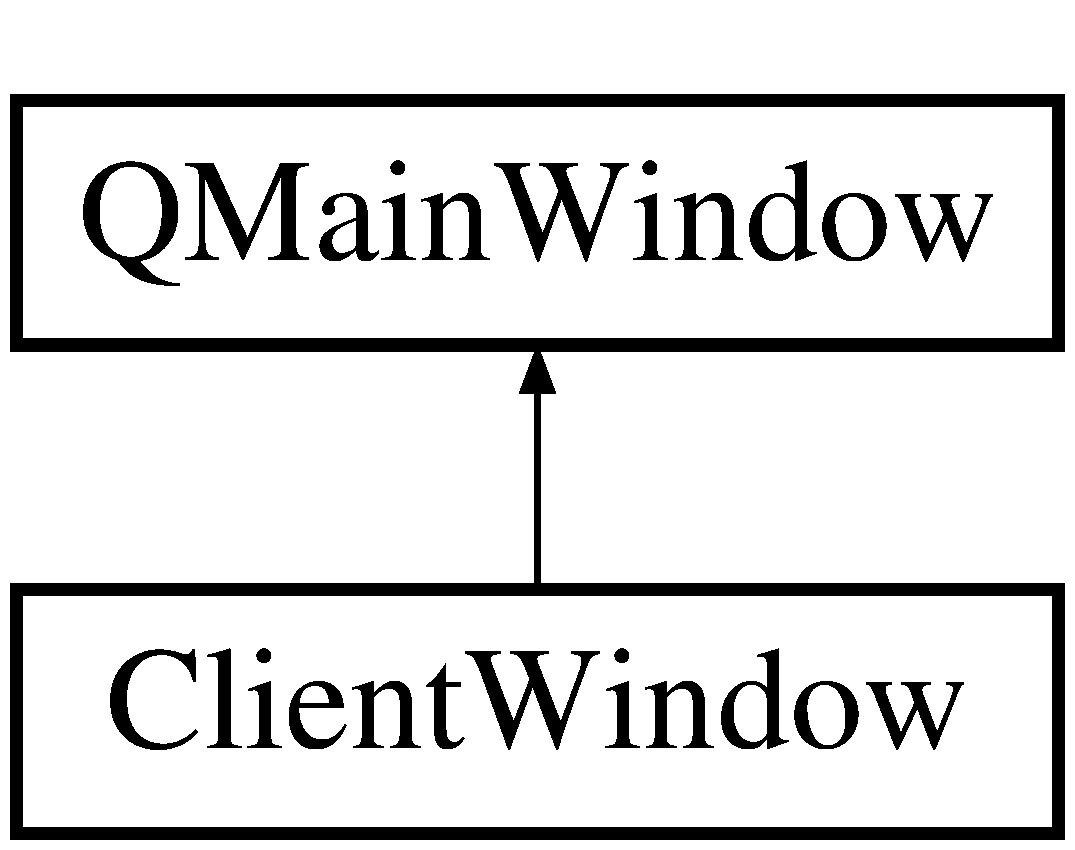
\includegraphics[height=2.000000cm]{class_client_window}
\end{center}
\end{figure}
\subsection*{Public Slots}
\begin{DoxyCompactItemize}
\item 
void \textbf{ on\+\_\+\+Search\+Line\+\_\+return\+Pressed} ()
\begin{DoxyCompactList}\small\item\em Слот, отвечающий за отправку поискового запроса на сервер по нажатию кнопки Return. \end{DoxyCompactList}\item 
void \textbf{ on\+Read} ()
\begin{DoxyCompactList}\small\item\em Слот, отвечающий за получение входящих данных \end{DoxyCompactList}\item 
void \textbf{ on\+\_\+\+Name\+Input\+\_\+return\+Pressed} ()
\begin{DoxyCompactList}\small\item\em Слот, отвечающий за сохранение и отправку на сервер имени пользователя \end{DoxyCompactList}\item 
void \textbf{ on\+\_\+\+Send\+Msg\+\_\+clicked} ()
\begin{DoxyCompactList}\small\item\em Слот, отвечающий за отправку сообщения пиру по нажатию (вызывает функцию отправки сообщения) \end{DoxyCompactList}\item 
void \textbf{ on\+\_\+\+Friend\+List\+\_\+item\+Double\+Clicked} (Q\+List\+Widget\+Item $\ast$item)
\begin{DoxyCompactList}\small\item\em Слот, определяющий имя пира, который был выбран пользователем (используется для отправки сообщений выбранному пользователю) \end{DoxyCompactList}\item 
void \textbf{ on\+\_\+\+Msg\+Input\+\_\+return\+Pressed} ()
\begin{DoxyCompactList}\small\item\em Слот, аналогичный \doxyref{on\+\_\+\+Send\+Msg\+\_\+clicked()}{p.}{class_client_window_a3868f97e58d97ea716137c52e50b968d}. Вызывает функцию отправки сообщения \end{DoxyCompactList}\item 
void \textbf{ Conn\+Detector} ()
\begin{DoxyCompactList}\small\item\em Слот для обнаружения входящих соединений \end{DoxyCompactList}\item 
void \textbf{ on\+\_\+\+Update\+List\+Button\+\_\+clicked} ()
\begin{DoxyCompactList}\small\item\em Слот, отвечающий за запрос серверу на получение списка всех пиров в сети. Активируется по нажатию кнопки Updated. \end{DoxyCompactList}\item 
void \textbf{ on\+\_\+check\+Box\+\_\+toggled} (bool checked)
\begin{DoxyCompactList}\small\item\em Слот, информирующий о нажатии галочки \char`\"{}\+Private\char`\"{} при входе в сеть. Устанавливает соответствующий статус(\+Private, Public)текущему пользователю \end{DoxyCompactList}\item 
void \textbf{ on\+\_\+push\+Button\+\_\+clicked} ()
\begin{DoxyCompactList}\small\item\em Слот для открытия Issue Creator по нажатию соответствующей кнопки \end{DoxyCompactList}\end{DoxyCompactItemize}
\subsection*{Public Member Functions}
\begin{DoxyCompactItemize}
\item 
\textbf{ Client\+Window} (int Port, Q\+String address, Q\+Widget $\ast$parent=0)
\begin{DoxyCompactList}\small\item\em Конструктор, принимающий на вход порт и адрес информационного сервера \end{DoxyCompactList}\item 
\textbf{ $\sim$\+Client\+Window} ()
\begin{DoxyCompactList}\small\item\em Деструктор \end{DoxyCompactList}\end{DoxyCompactItemize}
\subsection*{Private Member Functions}
\begin{DoxyCompactItemize}
\item 
int \textbf{ Resolver} (const Q\+String \&Data)
\begin{DoxyCompactList}\small\item\em Функция, предназначенная для распознавания типа данных, переданных в неё \end{DoxyCompactList}\item 
void \textbf{ Send\+Message\+To\+Peer} (const Q\+String \&Peer\+Name)
\begin{DoxyCompactList}\small\item\em Функция для отправки сообщения пиру \end{DoxyCompactList}\item 
void \textbf{ Connect\+To\+Peer} (const Q\+String \&IP, int Port, const Q\+String \&User\+Name)
\begin{DoxyCompactList}\small\item\em Функция для отправки запроса на соединение другому пиру \end{DoxyCompactList}\item 
void \textbf{ Send\+Connect\+Request} (const Q\+String \&Peer\+Name)
\begin{DoxyCompactList}\small\item\em Функция для отправки запроса на соединение другому пиру если статус текущего пользователя -\/ приватный. \end{DoxyCompactList}\item 
void \textbf{ Parse\+All\+Users\+Data} (Q\+String Response)
\begin{DoxyCompactList}\small\item\em Парсер списка пользователей, полученного от сервера \end{DoxyCompactList}\item 
Q\+String \textbf{ Encrypt} (Q\+String \&Message, Q\+String Key)
\begin{DoxyCompactList}\small\item\em Функция зашифровки сообщения с заданным ключом Функция шифрует сообщение по алгоритму \char`\"{}Кузнечик\char`\"{} (ГОСТ Р 34.\+12-\/2015) с заданным ключом. Подробнее ознакомиться с реализацией можно перейдя по ссылке в источниках. \end{DoxyCompactList}\item 
Q\+String \textbf{ Decrypt} (Q\+String \&Message, Q\+String Key)
\begin{DoxyCompactList}\small\item\em Функция расшифровки сообщения с заданным ключом Функция дешифрует сообщение по алгоритму \char`\"{}Кузнечик\char`\"{} (ГОСТ Р 34.\+12-\/2015) с заданным ключом. Подробнее ознакомиться с реализацией можно перейдя по ссылке в источниках. \end{DoxyCompactList}\item 
void \textbf{ Gen\+Key\+Params} ()
\begin{DoxyCompactList}\small\item\em Функция для генерации параметров ключей (Prime, Generator, Priv\+Numb, Public\+Numb) и самой пары ключей. \end{DoxyCompactList}\item 
Crypto\+P\+P\+::\+Sec\+Byte\+Block \textbf{ Incoming\+Session\+Key\+Gen} (const Q\+String \&Username, Crypto\+P\+P\+::\+Integer prime, Crypto\+P\+P\+::\+Integer generator, Crypto\+P\+P\+::\+Sec\+Byte\+Block public\+Numb)
\begin{DoxyCompactList}\small\item\em Функция для генерации параметров и выработки сеансового ключа с пиром, приславшим свои публичные данные для обмена ключами. \end{DoxyCompactList}\item 
void \textbf{ Getting\+Agreement} (const Q\+String \&Username, Crypto\+P\+P\+::\+Sec\+Byte\+Block public\+Numb)
\begin{DoxyCompactList}\small\item\em Функция для согласования общего сеансового ключа \end{DoxyCompactList}\item 
void \textbf{ Send\+Generated\+Public\+Key} (const Q\+String \&User\+Name, Crypto\+P\+P\+::\+Sec\+Byte\+Block public\+Key)
\begin{DoxyCompactList}\small\item\em Функция отправки публичного ключа заданному пиру \end{DoxyCompactList}\item 
\textbf{ Peer} $\ast$ \textbf{ Search\+Peer\+By\+Name} (const Q\+String \&Name)
\begin{DoxyCompactList}\small\item\em Функция поиска пира в структуре по имени. \end{DoxyCompactList}\end{DoxyCompactItemize}
\subsection*{Private Attributes}
\begin{DoxyCompactItemize}
\item 
Crypto\+P\+P\+::\+DH \textbf{ dh}
\begin{DoxyCompactList}\small\item\em Объект класса DH, необходимый для реализации алгоритма Диффи-\/Хеллмана. Подробнее можно узнать в официальной документации библиотеки Crypto\+PP. \end{DoxyCompactList}\item 
Crypto\+P\+P\+::\+Integer \textbf{ Prime}
\begin{DoxyCompactList}\small\item\em Параметр необходимый для генерации пары ключей. Подробнее можно узнать в официальной документации библиотеки Crypto\+PP. \end{DoxyCompactList}\item 
Crypto\+P\+P\+::\+Integer \textbf{ Generator}
\begin{DoxyCompactList}\small\item\em Параметр необходимый для генерации пары ключей. Подробнее можно узнать в официальной документации библиотеки Crypto\+PP. \end{DoxyCompactList}\item 
Crypto\+P\+P\+::\+Sec\+Byte\+Block \textbf{ Priv\+Numb}
\begin{DoxyCompactList}\small\item\em Публичное сгенерированное с помощью вышеуказанных параметров число. Подробнее можно узнать в официальной документации библиотеки Crypto\+PP. \end{DoxyCompactList}\item 
Crypto\+P\+P\+::\+Sec\+Byte\+Block \textbf{ Public\+Numb}
\begin{DoxyCompactList}\small\item\em Приватное сгенерированное с помощью вышеуказанных параметров число. Подробнее можно узнать в официальной документации библиотеки Crypto\+PP. \end{DoxyCompactList}\item 
Crypto\+P\+P\+::\+Sec\+Byte\+Block \textbf{ My\+Secret\+Key}
\begin{DoxyCompactList}\small\item\em Приватный ключ. Подробнее можно узнать в официальной документации библиотеки Crypto\+PP. \end{DoxyCompactList}\item 
Q\+Vector$<$ \textbf{ Peer} $>$ \textbf{ Peers}
\begin{DoxyCompactList}\small\item\em Структура для хранения списка известных пиров \end{DoxyCompactList}\item 
std\+::unique\+\_\+ptr$<$ Q\+Tcp\+Socket $>$ \textbf{ Server\+Socket}
\begin{DoxyCompactList}\small\item\em Указатель на сокет инициализированный адресом и портом информационного сервера \end{DoxyCompactList}\item 
std\+::unique\+\_\+ptr$<$ Q\+Tcp\+Server $>$ \textbf{ This\+Listen\+Socket}
\begin{DoxyCompactList}\small\item\em Указатель на слушающий сокет текущего пользователя \end{DoxyCompactList}\item 
Q\+String \textbf{ Destination}
\begin{DoxyCompactList}\small\item\em Имя адресата \end{DoxyCompactList}\item 
Q\+String \textbf{ Nick\+Name}
\begin{DoxyCompactList}\small\item\em Имя текущего пользователя \end{DoxyCompactList}\item 
Q\+String \textbf{ Server\+IP}
\begin{DoxyCompactList}\small\item\em I\+Pv4 адрес сервера \end{DoxyCompactList}\item 
int \textbf{ Server\+Port}
\begin{DoxyCompactList}\small\item\em Порт информационного сервера \end{DoxyCompactList}\item 
bool \textbf{ Connected\+To\+Server} = false
\begin{DoxyCompactList}\small\item\em Флаг, сигнализирующий о успешном присоединении к серверу. Если соединения нет -\/ поиск недоступен. \end{DoxyCompactList}\item 
bool \textbf{ Private} = false
\begin{DoxyCompactList}\small\item\em Флаг, сигнализирующий о статусе пользователя. \end{DoxyCompactList}\item 
Ui\+::\+Client\+Window $\ast$ \textbf{ ui}
\end{DoxyCompactItemize}


\subsection{Detailed Description}
Класс, предоставляющий интерфейc пользователя 

\subsection{Constructor \& Destructor Documentation}
\mbox{\label{class_client_window_a23d2aaa14ef2a3587252a32bca6ce9c4}} 
\index{Client\+Window@{Client\+Window}!Client\+Window@{Client\+Window}}
\index{Client\+Window@{Client\+Window}!Client\+Window@{Client\+Window}}
\subsubsection{Client\+Window()}
{\footnotesize\ttfamily Client\+Window\+::\+Client\+Window (\begin{DoxyParamCaption}\item[{int}]{Port,  }\item[{Q\+String}]{address,  }\item[{Q\+Widget $\ast$}]{parent = {\ttfamily 0} }\end{DoxyParamCaption})}



Конструктор, принимающий на вход порт и адрес информационного сервера 


\begin{DoxyParams}[1]{Parameters}
\mbox{\tt in}  & {\em Port} & Порт \\
\hline
\mbox{\tt in}  & {\em address} & I\+Pv4 адрес \\
\hline
\end{DoxyParams}
\mbox{\label{class_client_window_af98431ebb79bc205a7da60ada28ddb91}} 
\index{Client\+Window@{Client\+Window}!````~Client\+Window@{$\sim$\+Client\+Window}}
\index{````~Client\+Window@{$\sim$\+Client\+Window}!Client\+Window@{Client\+Window}}
\subsubsection{$\sim$\+Client\+Window()}
{\footnotesize\ttfamily Client\+Window\+::$\sim$\+Client\+Window (\begin{DoxyParamCaption}{ }\end{DoxyParamCaption})}



Деструктор 



\subsection{Member Function Documentation}
\mbox{\label{class_client_window_a1b54deb39018f95424f67e26c928db3f}} 
\index{Client\+Window@{Client\+Window}!Conn\+Detector@{Conn\+Detector}}
\index{Conn\+Detector@{Conn\+Detector}!Client\+Window@{Client\+Window}}
\subsubsection{Conn\+Detector}
{\footnotesize\ttfamily void Client\+Window\+::\+Conn\+Detector (\begin{DoxyParamCaption}{ }\end{DoxyParamCaption})\hspace{0.3cm}{\ttfamily [slot]}}



Слот для обнаружения входящих соединений 

\mbox{\label{class_client_window_a6a95a02873ba28363e00cb27d7e9cc6c}} 
\index{Client\+Window@{Client\+Window}!Connect\+To\+Peer@{Connect\+To\+Peer}}
\index{Connect\+To\+Peer@{Connect\+To\+Peer}!Client\+Window@{Client\+Window}}
\subsubsection{Connect\+To\+Peer()}
{\footnotesize\ttfamily void Client\+Window\+::\+Connect\+To\+Peer (\begin{DoxyParamCaption}\item[{const Q\+String \&}]{IP,  }\item[{int}]{Port,  }\item[{const Q\+String \&}]{User\+Name }\end{DoxyParamCaption})\hspace{0.3cm}{\ttfamily [private]}}



Функция для отправки запроса на соединение другому пиру 

Функция инициализирует новый сокет переданными данными (IP, Port), создается новый объект класса \doxyref{Peer}{p.}{class_peer}, использующийся для хранения данных о пользователе, заносит объект в структуру для хранения списка \char`\"{}знакомых\char`\"{} пиров, после чего этому пиру автоматически отправляется запрос на соединение. Получив такой запрос, пир автоматически сохранит пользователя отправившего этот запрос в своей структуре и сможет отправлять ему сообщения. Таким образом пиры будут \char`\"{}знать\char`\"{} друг друга без помощи информационного сервера 
\begin{DoxyParams}[1]{Parameters}
\mbox{\tt in}  & {\em IP} & I\+Pv4 адрес пира, которому будет отправляться запрос. \\
\hline
\mbox{\tt in}  & {\em Port} & Порт \\
\hline
\mbox{\tt in}  & {\em User\+Name} & Имя пира \\
\hline
\end{DoxyParams}
\begin{DoxyReturn}{Returns}
Ничего не возвращает 
\end{DoxyReturn}
\mbox{\label{class_client_window_ad577402b282f11ee0be8e1772acc9d8c}} 
\index{Client\+Window@{Client\+Window}!Decrypt@{Decrypt}}
\index{Decrypt@{Decrypt}!Client\+Window@{Client\+Window}}
\subsubsection{Decrypt()}
{\footnotesize\ttfamily Q\+String Client\+Window\+::\+Decrypt (\begin{DoxyParamCaption}\item[{Q\+String \&}]{Message,  }\item[{Q\+String}]{Key }\end{DoxyParamCaption})\hspace{0.3cm}{\ttfamily [private]}}



Функция расшифровки сообщения с заданным ключом Функция дешифрует сообщение по алгоритму \char`\"{}Кузнечик\char`\"{} (ГОСТ Р 34.\+12-\/2015) с заданным ключом. Подробнее ознакомиться с реализацией можно перейдя по ссылке в источниках. 


\begin{DoxyParams}[1]{Parameters}
\mbox{\tt in}  & {\em Message} & Сообщение, которое необходимо дешифровать. \\
\hline
\mbox{\tt in}  & {\em Key} & Ключ для дешифровки /return Возвращает строку -\/ расшифрованное сообщение \\
\hline
\end{DoxyParams}
\mbox{\label{class_client_window_a1d4012db90be784b11e1eda58202582c}} 
\index{Client\+Window@{Client\+Window}!Encrypt@{Encrypt}}
\index{Encrypt@{Encrypt}!Client\+Window@{Client\+Window}}
\subsubsection{Encrypt()}
{\footnotesize\ttfamily Q\+String Client\+Window\+::\+Encrypt (\begin{DoxyParamCaption}\item[{Q\+String \&}]{Message,  }\item[{Q\+String}]{Key }\end{DoxyParamCaption})\hspace{0.3cm}{\ttfamily [private]}}



Функция зашифровки сообщения с заданным ключом Функция шифрует сообщение по алгоритму \char`\"{}Кузнечик\char`\"{} (ГОСТ Р 34.\+12-\/2015) с заданным ключом. Подробнее ознакомиться с реализацией можно перейдя по ссылке в источниках. 


\begin{DoxyParams}[1]{Parameters}
\mbox{\tt in}  & {\em Message} & Сообщение, которое необходимо зашифровать. \\
\hline
\mbox{\tt in}  & {\em Key} & Ключ для зашифровки \\
\hline
\end{DoxyParams}
\begin{DoxyReturn}{Returns}
Возвращает строку -\/ зашифрованное сообщение 
\end{DoxyReturn}
\mbox{\label{class_client_window_a80e1035659b8f9867ac4c40920617cec}} 
\index{Client\+Window@{Client\+Window}!Gen\+Key\+Params@{Gen\+Key\+Params}}
\index{Gen\+Key\+Params@{Gen\+Key\+Params}!Client\+Window@{Client\+Window}}
\subsubsection{Gen\+Key\+Params()}
{\footnotesize\ttfamily void Client\+Window\+::\+Gen\+Key\+Params (\begin{DoxyParamCaption}{ }\end{DoxyParamCaption})\hspace{0.3cm}{\ttfamily [private]}}



Функция для генерации параметров ключей (Prime, Generator, Priv\+Numb, Public\+Numb) и самой пары ключей. 

Подробнее о параметрах можно прочесть в описании алгоритма Диффи-\/Хеллмана. \begin{DoxyReturn}{Returns}
Ничего не возвращает 
\end{DoxyReturn}
\mbox{\label{class_client_window_ad44d1603d88233c0f18dba2f64198da1}} 
\index{Client\+Window@{Client\+Window}!Getting\+Agreement@{Getting\+Agreement}}
\index{Getting\+Agreement@{Getting\+Agreement}!Client\+Window@{Client\+Window}}
\subsubsection{Getting\+Agreement()}
{\footnotesize\ttfamily void Client\+Window\+::\+Getting\+Agreement (\begin{DoxyParamCaption}\item[{const Q\+String \&}]{Username,  }\item[{Crypto\+P\+P\+::\+Sec\+Byte\+Block}]{public\+Numb }\end{DoxyParamCaption})\hspace{0.3cm}{\ttfamily [private]}}



Функция для согласования общего сеансового ключа 

С помощью полученного от пира его публичного ключа, сеансовый ключ согласуется и заносится в структру этого пира для последующей шифровки и дешифровки сообщений. 
\begin{DoxyParams}[1]{Parameters}
\mbox{\tt in}  & {\em Username} & Имя пира \\
\hline
\mbox{\tt in}  & {\em public\+Numb} & Публичный ключ, полученный пиром, приславшим запрос, при выработке сеансового ключа. \\
\hline
\end{DoxyParams}
\begin{DoxyReturn}{Returns}
Ничего не возвращает 
\end{DoxyReturn}
\mbox{\label{class_client_window_aeef0e4f3943b8d83aba3d8f1f784562b}} 
\index{Client\+Window@{Client\+Window}!Incoming\+Session\+Key\+Gen@{Incoming\+Session\+Key\+Gen}}
\index{Incoming\+Session\+Key\+Gen@{Incoming\+Session\+Key\+Gen}!Client\+Window@{Client\+Window}}
\subsubsection{Incoming\+Session\+Key\+Gen()}
{\footnotesize\ttfamily Crypto\+P\+P\+::\+Sec\+Byte\+Block Client\+Window\+::\+Incoming\+Session\+Key\+Gen (\begin{DoxyParamCaption}\item[{const Q\+String \&}]{Username,  }\item[{Crypto\+P\+P\+::\+Integer}]{prime,  }\item[{Crypto\+P\+P\+::\+Integer}]{generator,  }\item[{Crypto\+P\+P\+::\+Sec\+Byte\+Block}]{public\+Numb }\end{DoxyParamCaption})\hspace{0.3cm}{\ttfamily [private]}}



Функция для генерации параметров и выработки сеансового ключа с пиром, приславшим свои публичные данные для обмена ключами. 

Вызывается при получении запроса от пира на обмен ключами. Все необходимые данные он предоставляет в запросе. Подробнее о необходимых параметрах можно прочесть в описании алгоритма Диффи-\/Хеллмана. После генерации ключ заносится в структуру этого пира для последующей шифровки и дешифровки сообщений. 
\begin{DoxyParams}[1]{Parameters}
\mbox{\tt in}  & {\em Username} & Имя пира \\
\hline
\mbox{\tt in}  & {\em prime} & Prime параметр \\
\hline
\mbox{\tt in}  & {\em generator} & Generator параметр \\
\hline
\mbox{\tt in}  & {\em public\+Numb} & Публичный ключ, полученный пиром, приславшим запрос, при выработке ключа. \\
\hline
\end{DoxyParams}
\begin{DoxyReturn}{Returns}
Возвращает сеансовый ключ для данного пира 
\end{DoxyReturn}
\mbox{\label{class_client_window_a9d4b9f1e07bd287fcf7acbe62ab1efd3}} 
\index{Client\+Window@{Client\+Window}!on\+\_\+check\+Box\+\_\+toggled@{on\+\_\+check\+Box\+\_\+toggled}}
\index{on\+\_\+check\+Box\+\_\+toggled@{on\+\_\+check\+Box\+\_\+toggled}!Client\+Window@{Client\+Window}}
\subsubsection{on\+\_\+check\+Box\+\_\+toggled}
{\footnotesize\ttfamily void Client\+Window\+::on\+\_\+check\+Box\+\_\+toggled (\begin{DoxyParamCaption}\item[{bool}]{checked }\end{DoxyParamCaption})\hspace{0.3cm}{\ttfamily [slot]}}



Слот, информирующий о нажатии галочки \char`\"{}\+Private\char`\"{} при входе в сеть. Устанавливает соответствующий статус(\+Private, Public)текущему пользователю 

\mbox{\label{class_client_window_a53683c81555a53e513066619a66bdbf4}} 
\index{Client\+Window@{Client\+Window}!on\+\_\+\+Friend\+List\+\_\+item\+Double\+Clicked@{on\+\_\+\+Friend\+List\+\_\+item\+Double\+Clicked}}
\index{on\+\_\+\+Friend\+List\+\_\+item\+Double\+Clicked@{on\+\_\+\+Friend\+List\+\_\+item\+Double\+Clicked}!Client\+Window@{Client\+Window}}
\subsubsection{on\+\_\+\+Friend\+List\+\_\+item\+Double\+Clicked}
{\footnotesize\ttfamily void Client\+Window\+::on\+\_\+\+Friend\+List\+\_\+item\+Double\+Clicked (\begin{DoxyParamCaption}\item[{Q\+List\+Widget\+Item $\ast$}]{item }\end{DoxyParamCaption})\hspace{0.3cm}{\ttfamily [slot]}}



Слот, определяющий имя пира, который был выбран пользователем (используется для отправки сообщений выбранному пользователю) 

\mbox{\label{class_client_window_a201f45c14dfb71277f628ea6607d2959}} 
\index{Client\+Window@{Client\+Window}!on\+\_\+\+Msg\+Input\+\_\+return\+Pressed@{on\+\_\+\+Msg\+Input\+\_\+return\+Pressed}}
\index{on\+\_\+\+Msg\+Input\+\_\+return\+Pressed@{on\+\_\+\+Msg\+Input\+\_\+return\+Pressed}!Client\+Window@{Client\+Window}}
\subsubsection{on\+\_\+\+Msg\+Input\+\_\+return\+Pressed}
{\footnotesize\ttfamily void Client\+Window\+::on\+\_\+\+Msg\+Input\+\_\+return\+Pressed (\begin{DoxyParamCaption}{ }\end{DoxyParamCaption})\hspace{0.3cm}{\ttfamily [slot]}}



Слот, аналогичный \doxyref{on\+\_\+\+Send\+Msg\+\_\+clicked()}{p.}{class_client_window_a3868f97e58d97ea716137c52e50b968d}. Вызывает функцию отправки сообщения 

\mbox{\label{class_client_window_ac2bce105ea893651dc9daf567bb966b5}} 
\index{Client\+Window@{Client\+Window}!on\+\_\+\+Name\+Input\+\_\+return\+Pressed@{on\+\_\+\+Name\+Input\+\_\+return\+Pressed}}
\index{on\+\_\+\+Name\+Input\+\_\+return\+Pressed@{on\+\_\+\+Name\+Input\+\_\+return\+Pressed}!Client\+Window@{Client\+Window}}
\subsubsection{on\+\_\+\+Name\+Input\+\_\+return\+Pressed}
{\footnotesize\ttfamily void Client\+Window\+::on\+\_\+\+Name\+Input\+\_\+return\+Pressed (\begin{DoxyParamCaption}{ }\end{DoxyParamCaption})\hspace{0.3cm}{\ttfamily [slot]}}



Слот, отвечающий за сохранение и отправку на сервер имени пользователя 

\mbox{\label{class_client_window_ab8699235cbe5cc75a3180fdee7fb195c}} 
\index{Client\+Window@{Client\+Window}!on\+\_\+push\+Button\+\_\+clicked@{on\+\_\+push\+Button\+\_\+clicked}}
\index{on\+\_\+push\+Button\+\_\+clicked@{on\+\_\+push\+Button\+\_\+clicked}!Client\+Window@{Client\+Window}}
\subsubsection{on\+\_\+push\+Button\+\_\+clicked}
{\footnotesize\ttfamily void Client\+Window\+::on\+\_\+push\+Button\+\_\+clicked (\begin{DoxyParamCaption}{ }\end{DoxyParamCaption})\hspace{0.3cm}{\ttfamily [slot]}}



Слот для открытия Issue Creator по нажатию соответствующей кнопки 

\mbox{\label{class_client_window_a09a50177ec2bfc59fc9ec8f698153111}} 
\index{Client\+Window@{Client\+Window}!on\+\_\+\+Search\+Line\+\_\+return\+Pressed@{on\+\_\+\+Search\+Line\+\_\+return\+Pressed}}
\index{on\+\_\+\+Search\+Line\+\_\+return\+Pressed@{on\+\_\+\+Search\+Line\+\_\+return\+Pressed}!Client\+Window@{Client\+Window}}
\subsubsection{on\+\_\+\+Search\+Line\+\_\+return\+Pressed}
{\footnotesize\ttfamily void Client\+Window\+::on\+\_\+\+Search\+Line\+\_\+return\+Pressed (\begin{DoxyParamCaption}{ }\end{DoxyParamCaption})\hspace{0.3cm}{\ttfamily [slot]}}



Слот, отвечающий за отправку поискового запроса на сервер по нажатию кнопки Return. 

\mbox{\label{class_client_window_a3868f97e58d97ea716137c52e50b968d}} 
\index{Client\+Window@{Client\+Window}!on\+\_\+\+Send\+Msg\+\_\+clicked@{on\+\_\+\+Send\+Msg\+\_\+clicked}}
\index{on\+\_\+\+Send\+Msg\+\_\+clicked@{on\+\_\+\+Send\+Msg\+\_\+clicked}!Client\+Window@{Client\+Window}}
\subsubsection{on\+\_\+\+Send\+Msg\+\_\+clicked}
{\footnotesize\ttfamily void Client\+Window\+::on\+\_\+\+Send\+Msg\+\_\+clicked (\begin{DoxyParamCaption}{ }\end{DoxyParamCaption})\hspace{0.3cm}{\ttfamily [slot]}}



Слот, отвечающий за отправку сообщения пиру по нажатию (вызывает функцию отправки сообщения) 

\mbox{\label{class_client_window_a03213f4bad0ff25e75eeb617b61d5bdf}} 
\index{Client\+Window@{Client\+Window}!on\+\_\+\+Update\+List\+Button\+\_\+clicked@{on\+\_\+\+Update\+List\+Button\+\_\+clicked}}
\index{on\+\_\+\+Update\+List\+Button\+\_\+clicked@{on\+\_\+\+Update\+List\+Button\+\_\+clicked}!Client\+Window@{Client\+Window}}
\subsubsection{on\+\_\+\+Update\+List\+Button\+\_\+clicked}
{\footnotesize\ttfamily void Client\+Window\+::on\+\_\+\+Update\+List\+Button\+\_\+clicked (\begin{DoxyParamCaption}{ }\end{DoxyParamCaption})\hspace{0.3cm}{\ttfamily [slot]}}



Слот, отвечающий за запрос серверу на получение списка всех пиров в сети. Активируется по нажатию кнопки Updated. 

\mbox{\label{class_client_window_a6af59313228995e6c55d265db7ce3995}} 
\index{Client\+Window@{Client\+Window}!on\+Read@{on\+Read}}
\index{on\+Read@{on\+Read}!Client\+Window@{Client\+Window}}
\subsubsection{on\+Read}
{\footnotesize\ttfamily void Client\+Window\+::on\+Read (\begin{DoxyParamCaption}{ }\end{DoxyParamCaption})\hspace{0.3cm}{\ttfamily [slot]}}



Слот, отвечающий за получение входящих данных 

Передает данные в Resolver, который вернет информацию о формате пришедших данных. После определения формата (сообщение, ответ от сервера, запрос на обмен ключами и т.\+п.) -\/ функция передает данные на обработку \mbox{\label{class_client_window_adef4d0491b4ac3d7f4066acfef0841c4}} 
\index{Client\+Window@{Client\+Window}!Parse\+All\+Users\+Data@{Parse\+All\+Users\+Data}}
\index{Parse\+All\+Users\+Data@{Parse\+All\+Users\+Data}!Client\+Window@{Client\+Window}}
\subsubsection{Parse\+All\+Users\+Data()}
{\footnotesize\ttfamily void Client\+Window\+::\+Parse\+All\+Users\+Data (\begin{DoxyParamCaption}\item[{Q\+String}]{Response }\end{DoxyParamCaption})\hspace{0.3cm}{\ttfamily [private]}}



Парсер списка пользователей, полученного от сервера 

Выполняет парсинг полученной на вход строки, после чего заносит каждого пользователя в структуру. Вызывается при входе в сеть, либо при обновлении всего списка [in] Response Строка, содержащая информацию обо всех пользователях в сети \begin{DoxyReturn}{Returns}
Ничего не возвращает 
\end{DoxyReturn}
\mbox{\label{class_client_window_af38cd3b6f4d7e7ab2c805460a95d3172}} 
\index{Client\+Window@{Client\+Window}!Resolver@{Resolver}}
\index{Resolver@{Resolver}!Client\+Window@{Client\+Window}}
\subsubsection{Resolver()}
{\footnotesize\ttfamily int Client\+Window\+::\+Resolver (\begin{DoxyParamCaption}\item[{const Q\+String \&}]{Data }\end{DoxyParamCaption})\hspace{0.3cm}{\ttfamily [private]}}



Функция, предназначенная для распознавания типа данных, переданных в неё 

Функция определяет приписанный к началу данных флаг, который указывает на тип данных (сообщение, ответ от сервера, различные запросы от других пиров). 
\begin{DoxyParams}[1]{Parameters}
\mbox{\tt in}  & {\em Data} & Данные, тип которых необходимо определить \\
\hline
\end{DoxyParams}
\begin{DoxyReturn}{Returns}
Число -\/ код, соответствующий типу пришедших данных. 
\end{DoxyReturn}
\mbox{\label{class_client_window_a040d239df2ae3f017b371ed2367642e5}} 
\index{Client\+Window@{Client\+Window}!Search\+Peer\+By\+Name@{Search\+Peer\+By\+Name}}
\index{Search\+Peer\+By\+Name@{Search\+Peer\+By\+Name}!Client\+Window@{Client\+Window}}
\subsubsection{Search\+Peer\+By\+Name()}
{\footnotesize\ttfamily \textbf{ Peer} $\ast$ Client\+Window\+::\+Search\+Peer\+By\+Name (\begin{DoxyParamCaption}\item[{const Q\+String \&}]{Name }\end{DoxyParamCaption})\hspace{0.3cm}{\ttfamily [private]}}



Функция поиска пира в структуре по имени. 


\begin{DoxyParams}[1]{Parameters}
\mbox{\tt in}  & {\em Name} & Имя искомого пира \\
\hline
\end{DoxyParams}
\begin{DoxyReturn}{Returns}
Возвращает указатель на объект пира 
\end{DoxyReturn}
\mbox{\label{class_client_window_a8c4913533d66f626237a353e98b81d69}} 
\index{Client\+Window@{Client\+Window}!Send\+Connect\+Request@{Send\+Connect\+Request}}
\index{Send\+Connect\+Request@{Send\+Connect\+Request}!Client\+Window@{Client\+Window}}
\subsubsection{Send\+Connect\+Request()}
{\footnotesize\ttfamily void Client\+Window\+::\+Send\+Connect\+Request (\begin{DoxyParamCaption}\item[{const Q\+String \&}]{Peer\+Name }\end{DoxyParamCaption})\hspace{0.3cm}{\ttfamily [private]}}



Функция для отправки запроса на соединение другому пиру если статус текущего пользователя -\/ приватный. 

Запрос на соединение не должен отправляться от приватного пира без необходимости, чтобы не раскрывать его. Если такая необходимость появляется -\/ запрос отправляется, тогда адресат будет знать приватного пользователя. 
\begin{DoxyParams}[1]{Parameters}
\mbox{\tt in}  & {\em User\+Name} & Имя пира (необходимо для поиска его в своей структуре, так как приватный пир имеет информацию обо всех публичных, соответственно они есть в его структуре, остается их только найти) \\
\hline
\end{DoxyParams}
\begin{DoxyReturn}{Returns}
Ничего не возвращает 
\end{DoxyReturn}
\mbox{\label{class_client_window_a64b8023ab0edf40ea745b667039846e6}} 
\index{Client\+Window@{Client\+Window}!Send\+Generated\+Public\+Key@{Send\+Generated\+Public\+Key}}
\index{Send\+Generated\+Public\+Key@{Send\+Generated\+Public\+Key}!Client\+Window@{Client\+Window}}
\subsubsection{Send\+Generated\+Public\+Key()}
{\footnotesize\ttfamily void Client\+Window\+::\+Send\+Generated\+Public\+Key (\begin{DoxyParamCaption}\item[{const Q\+String \&}]{User\+Name,  }\item[{Crypto\+P\+P\+::\+Sec\+Byte\+Block}]{public\+Key }\end{DoxyParamCaption})\hspace{0.3cm}{\ttfamily [private]}}



Функция отправки публичного ключа заданному пиру 


\begin{DoxyParams}[1]{Parameters}
\mbox{\tt in}  & {\em User\+Name} & Имя пира \\
\hline
\mbox{\tt in}  & {\em public\+Key} & Публичный ключ для отправки \\
\hline
\end{DoxyParams}
\begin{DoxyReturn}{Returns}
Ничего не возвращает 
\end{DoxyReturn}
\mbox{\label{class_client_window_a1da98989dfae2558359e2bfe0a87f03d}} 
\index{Client\+Window@{Client\+Window}!Send\+Message\+To\+Peer@{Send\+Message\+To\+Peer}}
\index{Send\+Message\+To\+Peer@{Send\+Message\+To\+Peer}!Client\+Window@{Client\+Window}}
\subsubsection{Send\+Message\+To\+Peer()}
{\footnotesize\ttfamily void Client\+Window\+::\+Send\+Message\+To\+Peer (\begin{DoxyParamCaption}\item[{const Q\+String \&}]{Peer\+Name }\end{DoxyParamCaption})\hspace{0.3cm}{\ttfamily [private]}}



Функция для отправки сообщения пиру 

Функция ищет нужного пира в списке пиров и отправляет ему введенное в окне ввода сообщение 
\begin{DoxyParams}[1]{Parameters}
\mbox{\tt in}  & {\em Peer\+Name} & Имя адресата \\
\hline
\end{DoxyParams}
\begin{DoxyReturn}{Returns}
Ничего не возвращает 
\end{DoxyReturn}


\subsection{Member Data Documentation}
\mbox{\label{class_client_window_a060cbd4e58c77c64edb9b5dd69c8da7d}} 
\index{Client\+Window@{Client\+Window}!Connected\+To\+Server@{Connected\+To\+Server}}
\index{Connected\+To\+Server@{Connected\+To\+Server}!Client\+Window@{Client\+Window}}
\subsubsection{Connected\+To\+Server}
{\footnotesize\ttfamily bool Client\+Window\+::\+Connected\+To\+Server = false\hspace{0.3cm}{\ttfamily [private]}}



Флаг, сигнализирующий о успешном присоединении к серверу. Если соединения нет -\/ поиск недоступен. 

\mbox{\label{class_client_window_a98ff51a0d70a591431b56d5e001a51d9}} 
\index{Client\+Window@{Client\+Window}!Destination@{Destination}}
\index{Destination@{Destination}!Client\+Window@{Client\+Window}}
\subsubsection{Destination}
{\footnotesize\ttfamily Q\+String Client\+Window\+::\+Destination\hspace{0.3cm}{\ttfamily [private]}}



Имя адресата 

\mbox{\label{class_client_window_a70e338edd34ee5043c35c03c6da85190}} 
\index{Client\+Window@{Client\+Window}!dh@{dh}}
\index{dh@{dh}!Client\+Window@{Client\+Window}}
\subsubsection{dh}
{\footnotesize\ttfamily Crypto\+P\+P\+::\+DH Client\+Window\+::dh\hspace{0.3cm}{\ttfamily [private]}}



Объект класса DH, необходимый для реализации алгоритма Диффи-\/Хеллмана. Подробнее можно узнать в официальной документации библиотеки Crypto\+PP. 

\mbox{\label{class_client_window_a72c4ff89452aba7e047970ad83c51369}} 
\index{Client\+Window@{Client\+Window}!Generator@{Generator}}
\index{Generator@{Generator}!Client\+Window@{Client\+Window}}
\subsubsection{Generator}
{\footnotesize\ttfamily Crypto\+P\+P\+::\+Integer Client\+Window\+::\+Generator\hspace{0.3cm}{\ttfamily [private]}}



Параметр необходимый для генерации пары ключей. Подробнее можно узнать в официальной документации библиотеки Crypto\+PP. 

\mbox{\label{class_client_window_a771a96af9209f03fab4db74ad343c280}} 
\index{Client\+Window@{Client\+Window}!My\+Secret\+Key@{My\+Secret\+Key}}
\index{My\+Secret\+Key@{My\+Secret\+Key}!Client\+Window@{Client\+Window}}
\subsubsection{My\+Secret\+Key}
{\footnotesize\ttfamily Crypto\+P\+P\+::\+Sec\+Byte\+Block Client\+Window\+::\+My\+Secret\+Key\hspace{0.3cm}{\ttfamily [private]}}



Приватный ключ. Подробнее можно узнать в официальной документации библиотеки Crypto\+PP. 

\mbox{\label{class_client_window_a0a1282c1054a3810a4c772db4ffde530}} 
\index{Client\+Window@{Client\+Window}!Nick\+Name@{Nick\+Name}}
\index{Nick\+Name@{Nick\+Name}!Client\+Window@{Client\+Window}}
\subsubsection{Nick\+Name}
{\footnotesize\ttfamily Q\+String Client\+Window\+::\+Nick\+Name\hspace{0.3cm}{\ttfamily [private]}}



Имя текущего пользователя 

\mbox{\label{class_client_window_a8e6109e2659c78a3f959df0a450862ae}} 
\index{Client\+Window@{Client\+Window}!Peers@{Peers}}
\index{Peers@{Peers}!Client\+Window@{Client\+Window}}
\subsubsection{Peers}
{\footnotesize\ttfamily Q\+Vector$<$\textbf{ Peer}$>$ Client\+Window\+::\+Peers\hspace{0.3cm}{\ttfamily [private]}}



Структура для хранения списка известных пиров 

\mbox{\label{class_client_window_aab318f5417f89201dc6633b2e481e817}} 
\index{Client\+Window@{Client\+Window}!Prime@{Prime}}
\index{Prime@{Prime}!Client\+Window@{Client\+Window}}
\subsubsection{Prime}
{\footnotesize\ttfamily Crypto\+P\+P\+::\+Integer Client\+Window\+::\+Prime\hspace{0.3cm}{\ttfamily [private]}}



Параметр необходимый для генерации пары ключей. Подробнее можно узнать в официальной документации библиотеки Crypto\+PP. 

\mbox{\label{class_client_window_a0112c19a3296b1908e823d9baaa2246b}} 
\index{Client\+Window@{Client\+Window}!Private@{Private}}
\index{Private@{Private}!Client\+Window@{Client\+Window}}
\subsubsection{Private}
{\footnotesize\ttfamily bool Client\+Window\+::\+Private = false\hspace{0.3cm}{\ttfamily [private]}}



Флаг, сигнализирующий о статусе пользователя. 

\mbox{\label{class_client_window_a4c4248eb0be6db957bbd835146e36699}} 
\index{Client\+Window@{Client\+Window}!Priv\+Numb@{Priv\+Numb}}
\index{Priv\+Numb@{Priv\+Numb}!Client\+Window@{Client\+Window}}
\subsubsection{Priv\+Numb}
{\footnotesize\ttfamily Crypto\+P\+P\+::\+Sec\+Byte\+Block Client\+Window\+::\+Priv\+Numb\hspace{0.3cm}{\ttfamily [private]}}



Публичное сгенерированное с помощью вышеуказанных параметров число. Подробнее можно узнать в официальной документации библиотеки Crypto\+PP. 

\mbox{\label{class_client_window_a213087869fc5bfb7427add5248e60046}} 
\index{Client\+Window@{Client\+Window}!Public\+Numb@{Public\+Numb}}
\index{Public\+Numb@{Public\+Numb}!Client\+Window@{Client\+Window}}
\subsubsection{Public\+Numb}
{\footnotesize\ttfamily Crypto\+P\+P\+::\+Sec\+Byte\+Block Client\+Window\+::\+Public\+Numb\hspace{0.3cm}{\ttfamily [private]}}



Приватное сгенерированное с помощью вышеуказанных параметров число. Подробнее можно узнать в официальной документации библиотеки Crypto\+PP. 

\mbox{\label{class_client_window_abaec733868dc94910f89011513ab4c7b}} 
\index{Client\+Window@{Client\+Window}!Server\+IP@{Server\+IP}}
\index{Server\+IP@{Server\+IP}!Client\+Window@{Client\+Window}}
\subsubsection{Server\+IP}
{\footnotesize\ttfamily Q\+String Client\+Window\+::\+Server\+IP\hspace{0.3cm}{\ttfamily [private]}}



I\+Pv4 адрес сервера 

\mbox{\label{class_client_window_a3f0c47409cc45b690b52ecf177a86adb}} 
\index{Client\+Window@{Client\+Window}!Server\+Port@{Server\+Port}}
\index{Server\+Port@{Server\+Port}!Client\+Window@{Client\+Window}}
\subsubsection{Server\+Port}
{\footnotesize\ttfamily int Client\+Window\+::\+Server\+Port\hspace{0.3cm}{\ttfamily [private]}}



Порт информационного сервера 

\mbox{\label{class_client_window_a74e7b0eb499506ff2071e314cdab83dc}} 
\index{Client\+Window@{Client\+Window}!Server\+Socket@{Server\+Socket}}
\index{Server\+Socket@{Server\+Socket}!Client\+Window@{Client\+Window}}
\subsubsection{Server\+Socket}
{\footnotesize\ttfamily std\+::unique\+\_\+ptr$<$Q\+Tcp\+Socket$>$ Client\+Window\+::\+Server\+Socket\hspace{0.3cm}{\ttfamily [private]}}



Указатель на сокет инициализированный адресом и портом информационного сервера 

\mbox{\label{class_client_window_acff726e7e30b6bb9fd190181fbea4835}} 
\index{Client\+Window@{Client\+Window}!This\+Listen\+Socket@{This\+Listen\+Socket}}
\index{This\+Listen\+Socket@{This\+Listen\+Socket}!Client\+Window@{Client\+Window}}
\subsubsection{This\+Listen\+Socket}
{\footnotesize\ttfamily std\+::unique\+\_\+ptr$<$Q\+Tcp\+Server$>$ Client\+Window\+::\+This\+Listen\+Socket\hspace{0.3cm}{\ttfamily [private]}}



Указатель на слушающий сокет текущего пользователя 

\mbox{\label{class_client_window_a1fbbfac70cc4e23f0d44ac209804bfc9}} 
\index{Client\+Window@{Client\+Window}!ui@{ui}}
\index{ui@{ui}!Client\+Window@{Client\+Window}}
\subsubsection{ui}
{\footnotesize\ttfamily Ui\+::\+Client\+Window$\ast$ Client\+Window\+::ui\hspace{0.3cm}{\ttfamily [private]}}



The documentation for this class was generated from the following files\+:\begin{DoxyCompactItemize}
\item 
/\+Users/antonukhanov/\+P2\+P-\/\+Chat/\+Client/\textbf{ clientwindow.\+h}\item 
/\+Users/antonukhanov/\+P2\+P-\/\+Chat/\+Client/\textbf{ clientwindow.\+cpp}\end{DoxyCompactItemize}

\section{issuecreator Class Reference}
\label{classissuecreator}\index{issuecreator@{issuecreator}}


Класс, предоставляющий интерфейc для создания Github Issues.  




{\ttfamily \#include $<$issuecreator.\+h$>$}

Inheritance diagram for issuecreator\+:\begin{figure}[H]
\begin{center}
\leavevmode
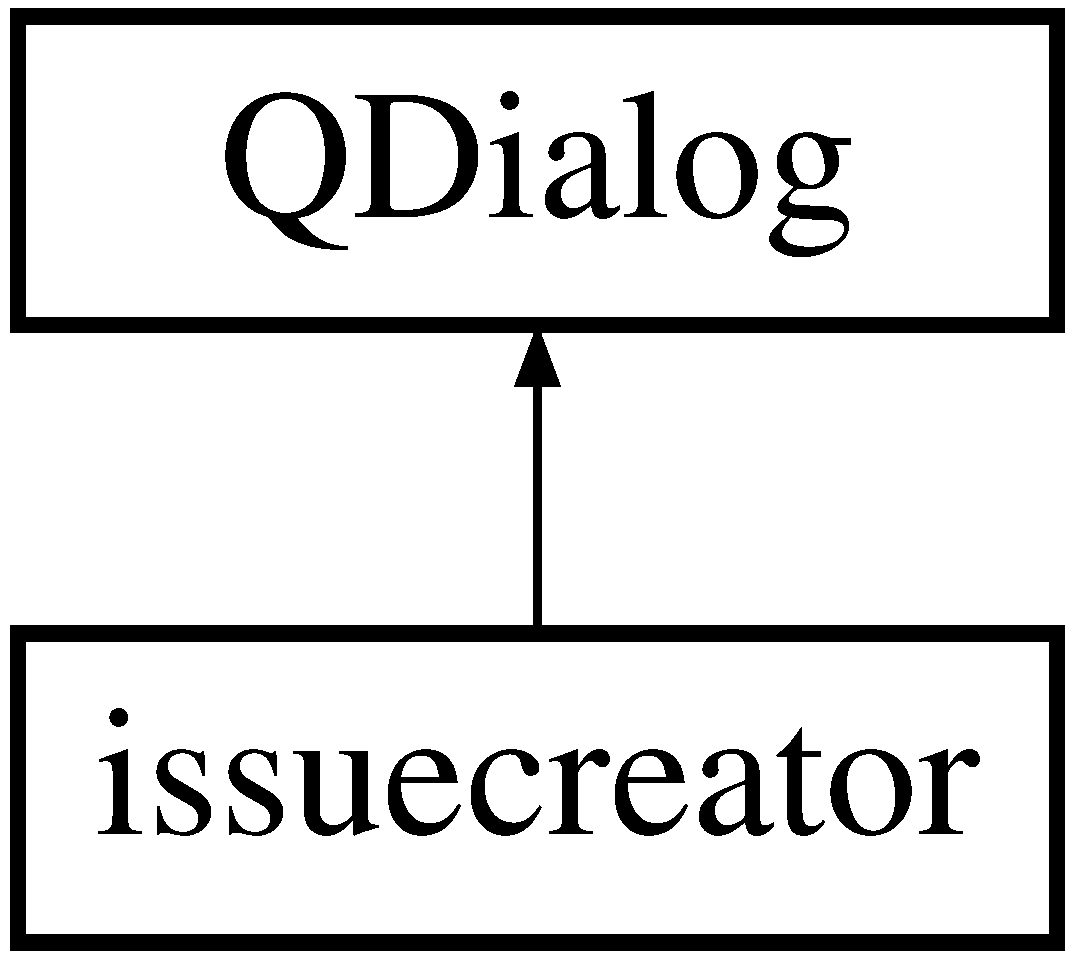
\includegraphics[height=2.000000cm]{classissuecreator}
\end{center}
\end{figure}
\subsection*{Public Member Functions}
\begin{DoxyCompactItemize}
\item 
\textbf{ issuecreator} (Q\+Widget $\ast$parent=0)
\begin{DoxyCompactList}\small\item\em Конструктор по умолчанию \end{DoxyCompactList}\item 
\textbf{ issuecreator} (const Q\+String \&selected\+Text, Q\+Widget $\ast$parent=0)
\begin{DoxyCompactList}\small\item\em Конструктор для случая с выделенным текстом. \end{DoxyCompactList}\item 
bool \textbf{ Is\+Internet\+Connected} ()
\begin{DoxyCompactList}\small\item\em Проверка интернет-\/соединения. Проверка соединения с помощью стандартных средств Qt. \end{DoxyCompactList}\item 
void \textbf{ Write\+Token\+To\+File} (const std\+::string \&\textbf{ Token})
\begin{DoxyCompactList}\small\item\em Запись в config-\/файл токена. \end{DoxyCompactList}\item 
Q\+String \textbf{ Read\+Token\+From\+File} ()
\begin{DoxyCompactList}\small\item\em Чтение токена из config-\/файла. \end{DoxyCompactList}\item 
Q\+String \textbf{ Parse\+Token} (Q\+String Data)
\begin{DoxyCompactList}\small\item\em Парсинг полученных данных от Github и получение токена из них. \end{DoxyCompactList}\item 
Q\+String \textbf{ Get\+Github\+Token} (const Q\+String \&Login, const Q\+String \&Pass)
\begin{DoxyCompactList}\small\item\em Отправка запроса на получение Github токена. \end{DoxyCompactList}\item 
\textbf{ $\sim$issuecreator} ()
\end{DoxyCompactItemize}
\subsection*{Private Slots}
\begin{DoxyCompactItemize}
\item 
void \textbf{ on\+\_\+\+Send\+\_\+clicked} ()
\begin{DoxyCompactList}\small\item\em Слот, отвечающий за отправку запроса на Github с целью создания Issue. \end{DoxyCompactList}\end{DoxyCompactItemize}
\subsection*{Private Attributes}
\begin{DoxyCompactItemize}
\item 
bool \textbf{ is\+Token\+Writed} = false
\begin{DoxyCompactList}\small\item\em Флаг, сигнализирующий о наличии токена в файле config. \end{DoxyCompactList}\item 
Q\+String \textbf{ Token}
\begin{DoxyCompactList}\small\item\em Токен \end{DoxyCompactList}\item 
Q\+String \textbf{ Issue\+Description}
\begin{DoxyCompactList}\small\item\em Описание проблемы \end{DoxyCompactList}\item 
Ui\+::issuecreator $\ast$ \textbf{ ui}
\end{DoxyCompactItemize}


\subsection{Detailed Description}
Класс, предоставляющий интерфейc для создания Github Issues. 

\subsection{Constructor \& Destructor Documentation}
\mbox{\label{classissuecreator_af18020b34fc69c9ffea22e7f748b8f96}} 
\index{issuecreator@{issuecreator}!issuecreator@{issuecreator}}
\index{issuecreator@{issuecreator}!issuecreator@{issuecreator}}
\subsubsection{issuecreator()\hspace{0.1cm}{\footnotesize\ttfamily [1/2]}}
{\footnotesize\ttfamily issuecreator\+::issuecreator (\begin{DoxyParamCaption}\item[{Q\+Widget $\ast$}]{parent = {\ttfamily 0} }\end{DoxyParamCaption})\hspace{0.3cm}{\ttfamily [explicit]}}



Конструктор по умолчанию 

\mbox{\label{classissuecreator_ae623be0a0b031f1382b844133e51e1cb}} 
\index{issuecreator@{issuecreator}!issuecreator@{issuecreator}}
\index{issuecreator@{issuecreator}!issuecreator@{issuecreator}}
\subsubsection{issuecreator()\hspace{0.1cm}{\footnotesize\ttfamily [2/2]}}
{\footnotesize\ttfamily issuecreator\+::issuecreator (\begin{DoxyParamCaption}\item[{const Q\+String \&}]{selected\+Text,  }\item[{Q\+Widget $\ast$}]{parent = {\ttfamily 0} }\end{DoxyParamCaption})}



Конструктор для случая с выделенным текстом. 

Весь выделенный текст в окне сообщений будет перенесен в панель ввода Description. \mbox{\label{classissuecreator_ac3f6c719cc0c836d709f92a166f5ee30}} 
\index{issuecreator@{issuecreator}!````~issuecreator@{$\sim$issuecreator}}
\index{````~issuecreator@{$\sim$issuecreator}!issuecreator@{issuecreator}}
\subsubsection{$\sim$issuecreator()}
{\footnotesize\ttfamily issuecreator\+::$\sim$issuecreator (\begin{DoxyParamCaption}{ }\end{DoxyParamCaption})}



\subsection{Member Function Documentation}
\mbox{\label{classissuecreator_a332d178719de5c6905603d4715fe179f}} 
\index{issuecreator@{issuecreator}!Get\+Github\+Token@{Get\+Github\+Token}}
\index{Get\+Github\+Token@{Get\+Github\+Token}!issuecreator@{issuecreator}}
\subsubsection{Get\+Github\+Token()}
{\footnotesize\ttfamily Q\+String issuecreator\+::\+Get\+Github\+Token (\begin{DoxyParamCaption}\item[{const Q\+String \&}]{Login,  }\item[{const Q\+String \&}]{Pass }\end{DoxyParamCaption})}



Отправка запроса на получение Github токена. 


\begin{DoxyParams}[1]{Parameters}
\mbox{\tt in}  & {\em Login} & Логин Github. \\
\hline
\mbox{\tt in}  & {\em Pass} & Пароль от аккаунта Github. \\
\hline
\end{DoxyParams}
\mbox{\label{classissuecreator_a9c4e6f82cc1c1523bbd92d38b35b75ad}} 
\index{issuecreator@{issuecreator}!Is\+Internet\+Connected@{Is\+Internet\+Connected}}
\index{Is\+Internet\+Connected@{Is\+Internet\+Connected}!issuecreator@{issuecreator}}
\subsubsection{Is\+Internet\+Connected()}
{\footnotesize\ttfamily bool issuecreator\+::\+Is\+Internet\+Connected (\begin{DoxyParamCaption}{ }\end{DoxyParamCaption})}



Проверка интернет-\/соединения. Проверка соединения с помощью стандартных средств Qt. 

\begin{DoxyReturn}{Returns}
False если отсутствует интернет-\/соединение. Иначе -\/ true. 
\end{DoxyReturn}
\mbox{\label{classissuecreator_a03af040ad19d02a8c271fe0c7b40d160}} 
\index{issuecreator@{issuecreator}!on\+\_\+\+Send\+\_\+clicked@{on\+\_\+\+Send\+\_\+clicked}}
\index{on\+\_\+\+Send\+\_\+clicked@{on\+\_\+\+Send\+\_\+clicked}!issuecreator@{issuecreator}}
\subsubsection{on\+\_\+\+Send\+\_\+clicked}
{\footnotesize\ttfamily void issuecreator\+::on\+\_\+\+Send\+\_\+clicked (\begin{DoxyParamCaption}{ }\end{DoxyParamCaption})\hspace{0.3cm}{\ttfamily [private]}, {\ttfamily [slot]}}



Слот, отвечающий за отправку запроса на Github с целью создания Issue. 

\mbox{\label{classissuecreator_a32184b3842bd6352faeef506b85c649a}} 
\index{issuecreator@{issuecreator}!Parse\+Token@{Parse\+Token}}
\index{Parse\+Token@{Parse\+Token}!issuecreator@{issuecreator}}
\subsubsection{Parse\+Token()}
{\footnotesize\ttfamily Q\+String issuecreator\+::\+Parse\+Token (\begin{DoxyParamCaption}\item[{Q\+String}]{Data }\end{DoxyParamCaption})}



Парсинг полученных данных от Github и получение токена из них. 


\begin{DoxyParams}[1]{Parameters}
\mbox{\tt in}  & {\em Data} & Данные от Github. \\
\hline
\end{DoxyParams}
\begin{DoxyReturn}{Returns}
Строка -\/ токен. 
\end{DoxyReturn}
\mbox{\label{classissuecreator_a52fc815f5dd3099817a1613f4af9de9b}} 
\index{issuecreator@{issuecreator}!Read\+Token\+From\+File@{Read\+Token\+From\+File}}
\index{Read\+Token\+From\+File@{Read\+Token\+From\+File}!issuecreator@{issuecreator}}
\subsubsection{Read\+Token\+From\+File()}
{\footnotesize\ttfamily Q\+String issuecreator\+::\+Read\+Token\+From\+File (\begin{DoxyParamCaption}{ }\end{DoxyParamCaption})}



Чтение токена из config-\/файла. 

\begin{DoxyReturn}{Returns}
Строка -\/ токен. 
\end{DoxyReturn}
\mbox{\label{classissuecreator_a7d8b501ffe33324bad13029113674d3d}} 
\index{issuecreator@{issuecreator}!Write\+Token\+To\+File@{Write\+Token\+To\+File}}
\index{Write\+Token\+To\+File@{Write\+Token\+To\+File}!issuecreator@{issuecreator}}
\subsubsection{Write\+Token\+To\+File()}
{\footnotesize\ttfamily void issuecreator\+::\+Write\+Token\+To\+File (\begin{DoxyParamCaption}\item[{const std\+::string \&}]{Token }\end{DoxyParamCaption})}



Запись в config-\/файл токена. 


\begin{DoxyParams}[1]{Parameters}
\mbox{\tt in}  & {\em Token} & Токен для записи в файл. \\
\hline
\end{DoxyParams}


\subsection{Member Data Documentation}
\mbox{\label{classissuecreator_a7d6bc72a5a8ddafa35e3d0e759918586}} 
\index{issuecreator@{issuecreator}!Issue\+Description@{Issue\+Description}}
\index{Issue\+Description@{Issue\+Description}!issuecreator@{issuecreator}}
\subsubsection{Issue\+Description}
{\footnotesize\ttfamily Q\+String issuecreator\+::\+Issue\+Description\hspace{0.3cm}{\ttfamily [private]}}



Описание проблемы 

\mbox{\label{classissuecreator_ab95a97a1a87dae8170bfaf0c95859413}} 
\index{issuecreator@{issuecreator}!is\+Token\+Writed@{is\+Token\+Writed}}
\index{is\+Token\+Writed@{is\+Token\+Writed}!issuecreator@{issuecreator}}
\subsubsection{is\+Token\+Writed}
{\footnotesize\ttfamily bool issuecreator\+::is\+Token\+Writed = false\hspace{0.3cm}{\ttfamily [private]}}



Флаг, сигнализирующий о наличии токена в файле config. 

\mbox{\label{classissuecreator_ad8f87f64c334987f0316a3d3191d55c8}} 
\index{issuecreator@{issuecreator}!Token@{Token}}
\index{Token@{Token}!issuecreator@{issuecreator}}
\subsubsection{Token}
{\footnotesize\ttfamily Q\+String issuecreator\+::\+Token\hspace{0.3cm}{\ttfamily [private]}}



Токен 

\mbox{\label{classissuecreator_ae85db2bae308918495f313ac058b006b}} 
\index{issuecreator@{issuecreator}!ui@{ui}}
\index{ui@{ui}!issuecreator@{issuecreator}}
\subsubsection{ui}
{\footnotesize\ttfamily Ui\+::issuecreator$\ast$ issuecreator\+::ui\hspace{0.3cm}{\ttfamily [private]}}



The documentation for this class was generated from the following files\+:\begin{DoxyCompactItemize}
\item 
/\+Users/antonukhanov/\+P2\+P-\/\+Chat/\+Client/\textbf{ issuecreator.\+h}\item 
/\+Users/antonukhanov/\+P2\+P-\/\+Chat/\+Client/\textbf{ issuecreator.\+cpp}\end{DoxyCompactItemize}

\section{Kuznyechik Class Reference}
\label{class_kuznyechik}\index{Kuznyechik@{Kuznyechik}}


Класс из библиотеки-\/реализации алгоритма \char`\"{}Кузнечик\char`\"{}. Ссылка на документацию -\/ в источниках.  




{\ttfamily \#include $<$Kuznyechik.\+hpp$>$}

\subsection*{Public Member Functions}
\begin{DoxyCompactItemize}
\item 
\textbf{ Kuznyechik} (const \textbf{ Byte\+Block} \&key)
\item 
\textbf{ Kuznyechik} (const \textbf{ Kuznyechik} \&rhs)
\item 
\textbf{ $\sim$\+Kuznyechik} ()
\item 
void \textbf{ encrypt} (const \textbf{ Byte\+Block} \&src, \textbf{ Byte\+Block} \&dst) const
\item 
void \textbf{ decrypt} (const \textbf{ Byte\+Block} \&src, \textbf{ Byte\+Block} \&dst) const
\end{DoxyCompactItemize}
\subsection*{Static Public Attributes}
\begin{DoxyCompactItemize}
\item 
static const int \textbf{ block\+\_\+lenght} \{\textbf{ B\+L\+O\+C\+K\+\_\+\+L\+E\+N\+G\+TH}\}
\end{DoxyCompactItemize}
\subsection*{Private Attributes}
\begin{DoxyCompactItemize}
\item 
std\+::vector$<$ \textbf{ Byte\+Block} $>$ \textbf{ keys}
\end{DoxyCompactItemize}
\subsection*{Static Private Attributes}
\begin{DoxyCompactItemize}
\item 
static bool \textbf{ is\+\_\+init} = false
\end{DoxyCompactItemize}


\subsection{Detailed Description}
Класс из библиотеки-\/реализации алгоритма \char`\"{}Кузнечик\char`\"{}. Ссылка на документацию -\/ в источниках. 

\subsection{Constructor \& Destructor Documentation}
\mbox{\label{class_kuznyechik_a3fa49cd54a47b9cc2d5a32beabd05264}} 
\index{Kuznyechik@{Kuznyechik}!Kuznyechik@{Kuznyechik}}
\index{Kuznyechik@{Kuznyechik}!Kuznyechik@{Kuznyechik}}
\subsubsection{Kuznyechik()\hspace{0.1cm}{\footnotesize\ttfamily [1/2]}}
{\footnotesize\ttfamily Kuznyechik\+::\+Kuznyechik (\begin{DoxyParamCaption}\item[{const \textbf{ Byte\+Block} \&}]{key }\end{DoxyParamCaption})}

\mbox{\label{class_kuznyechik_a8e3a616991d823600e38d4a974124d1d}} 
\index{Kuznyechik@{Kuznyechik}!Kuznyechik@{Kuznyechik}}
\index{Kuznyechik@{Kuznyechik}!Kuznyechik@{Kuznyechik}}
\subsubsection{Kuznyechik()\hspace{0.1cm}{\footnotesize\ttfamily [2/2]}}
{\footnotesize\ttfamily Kuznyechik\+::\+Kuznyechik (\begin{DoxyParamCaption}\item[{const \textbf{ Kuznyechik} \&}]{rhs }\end{DoxyParamCaption})}

\mbox{\label{class_kuznyechik_a0dab125f7a2ba66559ee611256985c45}} 
\index{Kuznyechik@{Kuznyechik}!````~Kuznyechik@{$\sim$\+Kuznyechik}}
\index{````~Kuznyechik@{$\sim$\+Kuznyechik}!Kuznyechik@{Kuznyechik}}
\subsubsection{$\sim$\+Kuznyechik()}
{\footnotesize\ttfamily Kuznyechik\+::$\sim$\+Kuznyechik (\begin{DoxyParamCaption}{ }\end{DoxyParamCaption})}



\subsection{Member Function Documentation}
\mbox{\label{class_kuznyechik_a8f699d0a38e8fa9c147d7b31d759bf26}} 
\index{Kuznyechik@{Kuznyechik}!decrypt@{decrypt}}
\index{decrypt@{decrypt}!Kuznyechik@{Kuznyechik}}
\subsubsection{decrypt()}
{\footnotesize\ttfamily void Kuznyechik\+::decrypt (\begin{DoxyParamCaption}\item[{const \textbf{ Byte\+Block} \&}]{src,  }\item[{\textbf{ Byte\+Block} \&}]{dst }\end{DoxyParamCaption}) const}

\mbox{\label{class_kuznyechik_ace290770ef015f19d6c0e06c66a4f29d}} 
\index{Kuznyechik@{Kuznyechik}!encrypt@{encrypt}}
\index{encrypt@{encrypt}!Kuznyechik@{Kuznyechik}}
\subsubsection{encrypt()}
{\footnotesize\ttfamily void Kuznyechik\+::encrypt (\begin{DoxyParamCaption}\item[{const \textbf{ Byte\+Block} \&}]{src,  }\item[{\textbf{ Byte\+Block} \&}]{dst }\end{DoxyParamCaption}) const}



\subsection{Member Data Documentation}
\mbox{\label{class_kuznyechik_acf61a43f8d6c726b0d334df98bdc0337}} 
\index{Kuznyechik@{Kuznyechik}!block\+\_\+lenght@{block\+\_\+lenght}}
\index{block\+\_\+lenght@{block\+\_\+lenght}!Kuznyechik@{Kuznyechik}}
\subsubsection{block\+\_\+lenght}
{\footnotesize\ttfamily const int Kuznyechik\+::block\+\_\+lenght \{\textbf{ B\+L\+O\+C\+K\+\_\+\+L\+E\+N\+G\+TH}\}\hspace{0.3cm}{\ttfamily [static]}}

\mbox{\label{class_kuznyechik_ad174f2e619e033cc9f29a265825aba41}} 
\index{Kuznyechik@{Kuznyechik}!is\+\_\+init@{is\+\_\+init}}
\index{is\+\_\+init@{is\+\_\+init}!Kuznyechik@{Kuznyechik}}
\subsubsection{is\+\_\+init}
{\footnotesize\ttfamily bool Kuznyechik\+::is\+\_\+init = false\hspace{0.3cm}{\ttfamily [static]}, {\ttfamily [private]}}

\mbox{\label{class_kuznyechik_a19e910dc6d7358b07ab733c31ae52b8d}} 
\index{Kuznyechik@{Kuznyechik}!keys@{keys}}
\index{keys@{keys}!Kuznyechik@{Kuznyechik}}
\subsubsection{keys}
{\footnotesize\ttfamily std\+::vector$<$\textbf{ Byte\+Block}$>$ Kuznyechik\+::keys\hspace{0.3cm}{\ttfamily [private]}}



The documentation for this class was generated from the following files\+:\begin{DoxyCompactItemize}
\item 
/\+Users/antonukhanov/\+P2\+P-\/\+Chat/\+Client/\textbf{ Kuznyechik.\+hpp}\item 
/\+Users/antonukhanov/\+P2\+P-\/\+Chat/\+Client/\textbf{ Kuznyechik.\+cpp}\end{DoxyCompactItemize}

\hypertarget{class_peer}{}\section{Peer Class Reference}
\label{class_peer}\index{Peer@{Peer}}


Класс, предоставляющий интерфейс для хранения данных о каждом \char`\"{}знакомом\char`\"{} пире  




{\ttfamily \#include $<$peer.\+h$>$}

\subsection*{Public Member Functions}
\begin{DoxyCompactItemize}
\item 
\hyperlink{class_peer_a9649fd34528cb532cded43d84a163371}{Peer} ()
\begin{DoxyCompactList}\small\item\em Конструктор по умолчанию \end{DoxyCompactList}\item 
\hyperlink{class_peer_ace891b7f4130166ef1a15e2f5f6698f6}{Peer} (Q\+String Name, std\+::shared\+\_\+ptr$<$ Q\+Tcp\+Socket $>$ Socket)
\begin{DoxyCompactList}\small\item\em Конструктор, принимающий имя пира и указатель на сокет, инициализированный его адресом \end{DoxyCompactList}\item 
\hyperlink{class_peer_aa72ba8fe59c6d161a87e398b40dd7f61}{Peer} (Q\+String Name, std\+::shared\+\_\+ptr$<$ Q\+Tcp\+Socket $>$ Socket, Q\+String Key)
\begin{DoxyCompactList}\small\item\em Конструктор, принимающий имя пира, указатель на сокет(инициализированный его адресом) и сеансовый ключ для этого пира \end{DoxyCompactList}\item 
void \hyperlink{class_peer_a761fedbe29868c9c3fb3b2c0f337b18b}{Set\+Session\+Key} (Q\+String Key)
\begin{DoxyCompactList}\small\item\em Set-\/функция для инициализации сеансового ключа этого пира \end{DoxyCompactList}\end{DoxyCompactItemize}
\subsection*{Public Attributes}
\begin{DoxyCompactItemize}
\item 
Q\+String \hyperlink{class_peer_a1b31ac7becfb809b03d1926bf5507f6f}{Peer\+Name}
\begin{DoxyCompactList}\small\item\em Имя пира \end{DoxyCompactList}\item 
std\+::shared\+\_\+ptr$<$ Q\+Tcp\+Socket $>$ \hyperlink{class_peer_aaf19f96ad1374f7381ed51baa7f00b77}{Peer\+Socket}
\begin{DoxyCompactList}\small\item\em Указатель на сокет, инициализированный адресом пира \end{DoxyCompactList}\item 
Q\+String \hyperlink{class_peer_a6d280927dbdbc71827fa03cea40b78a5}{Session\+Key}
\begin{DoxyCompactList}\small\item\em Сеансовый ключ для этого пира \end{DoxyCompactList}\end{DoxyCompactItemize}


\subsection{Detailed Description}
Класс, предоставляющий интерфейс для хранения данных о каждом \char`\"{}знакомом\char`\"{} пире 

\subsection{Constructor \& Destructor Documentation}
\mbox{\Hypertarget{class_peer_a9649fd34528cb532cded43d84a163371}\label{class_peer_a9649fd34528cb532cded43d84a163371}} 
\index{Peer@{Peer}!Peer@{Peer}}
\index{Peer@{Peer}!Peer@{Peer}}
\subsubsection{\texorpdfstring{Peer()}{Peer()}\hspace{0.1cm}{\footnotesize\ttfamily [1/3]}}
{\footnotesize\ttfamily Peer\+::\+Peer (\begin{DoxyParamCaption}{ }\end{DoxyParamCaption})}



Конструктор по умолчанию 

\mbox{\Hypertarget{class_peer_ace891b7f4130166ef1a15e2f5f6698f6}\label{class_peer_ace891b7f4130166ef1a15e2f5f6698f6}} 
\index{Peer@{Peer}!Peer@{Peer}}
\index{Peer@{Peer}!Peer@{Peer}}
\subsubsection{\texorpdfstring{Peer()}{Peer()}\hspace{0.1cm}{\footnotesize\ttfamily [2/3]}}
{\footnotesize\ttfamily Peer\+::\+Peer (\begin{DoxyParamCaption}\item[{Q\+String}]{Name,  }\item[{std\+::shared\+\_\+ptr$<$ Q\+Tcp\+Socket $>$}]{Socket }\end{DoxyParamCaption})}



Конструктор, принимающий имя пира и указатель на сокет, инициализированный его адресом 

\mbox{\Hypertarget{class_peer_aa72ba8fe59c6d161a87e398b40dd7f61}\label{class_peer_aa72ba8fe59c6d161a87e398b40dd7f61}} 
\index{Peer@{Peer}!Peer@{Peer}}
\index{Peer@{Peer}!Peer@{Peer}}
\subsubsection{\texorpdfstring{Peer()}{Peer()}\hspace{0.1cm}{\footnotesize\ttfamily [3/3]}}
{\footnotesize\ttfamily Peer\+::\+Peer (\begin{DoxyParamCaption}\item[{Q\+String}]{Name,  }\item[{std\+::shared\+\_\+ptr$<$ Q\+Tcp\+Socket $>$}]{Socket,  }\item[{Q\+String}]{Key }\end{DoxyParamCaption})}



Конструктор, принимающий имя пира, указатель на сокет(инициализированный его адресом) и сеансовый ключ для этого пира 



\subsection{Member Function Documentation}
\mbox{\Hypertarget{class_peer_a761fedbe29868c9c3fb3b2c0f337b18b}\label{class_peer_a761fedbe29868c9c3fb3b2c0f337b18b}} 
\index{Peer@{Peer}!Set\+Session\+Key@{Set\+Session\+Key}}
\index{Set\+Session\+Key@{Set\+Session\+Key}!Peer@{Peer}}
\subsubsection{\texorpdfstring{Set\+Session\+Key()}{SetSessionKey()}}
{\footnotesize\ttfamily void Peer\+::\+Set\+Session\+Key (\begin{DoxyParamCaption}\item[{Q\+String}]{Key }\end{DoxyParamCaption})}



Set-\/функция для инициализации сеансового ключа этого пира 



\subsection{Member Data Documentation}
\mbox{\Hypertarget{class_peer_a1b31ac7becfb809b03d1926bf5507f6f}\label{class_peer_a1b31ac7becfb809b03d1926bf5507f6f}} 
\index{Peer@{Peer}!Peer\+Name@{Peer\+Name}}
\index{Peer\+Name@{Peer\+Name}!Peer@{Peer}}
\subsubsection{\texorpdfstring{Peer\+Name}{PeerName}}
{\footnotesize\ttfamily Q\+String Peer\+::\+Peer\+Name}



Имя пира 

\mbox{\Hypertarget{class_peer_aaf19f96ad1374f7381ed51baa7f00b77}\label{class_peer_aaf19f96ad1374f7381ed51baa7f00b77}} 
\index{Peer@{Peer}!Peer\+Socket@{Peer\+Socket}}
\index{Peer\+Socket@{Peer\+Socket}!Peer@{Peer}}
\subsubsection{\texorpdfstring{Peer\+Socket}{PeerSocket}}
{\footnotesize\ttfamily std\+::shared\+\_\+ptr$<$Q\+Tcp\+Socket$>$ Peer\+::\+Peer\+Socket}



Указатель на сокет, инициализированный адресом пира 

\mbox{\Hypertarget{class_peer_a6d280927dbdbc71827fa03cea40b78a5}\label{class_peer_a6d280927dbdbc71827fa03cea40b78a5}} 
\index{Peer@{Peer}!Session\+Key@{Session\+Key}}
\index{Session\+Key@{Session\+Key}!Peer@{Peer}}
\subsubsection{\texorpdfstring{Session\+Key}{SessionKey}}
{\footnotesize\ttfamily Q\+String Peer\+::\+Session\+Key}



Сеансовый ключ для этого пира 



The documentation for this class was generated from the following files\+:\begin{DoxyCompactItemize}
\item 
P2\+P-\/\+Chat/\+Client/\hyperlink{peer_8h}{peer.\+h}\item 
P2\+P-\/\+Chat/\+Client/\hyperlink{peer_8cpp}{peer.\+cpp}\end{DoxyCompactItemize}

\chapter{File Documentation}
\hypertarget{clientwindow_8cpp}{}\section{P2\+P-\/\+Chat/\+Client/clientwindow.cpp File Reference}
\label{clientwindow_8cpp}\index{P2\+P-\/\+Chat/\+Client/clientwindow.\+cpp@{P2\+P-\/\+Chat/\+Client/clientwindow.\+cpp}}
{\ttfamily \#include \char`\"{}clientwindow.\+h\char`\"{}}\newline
{\ttfamily \#include \char`\"{}ui\+\_\+clientwindow.\+h\char`\"{}}\newline
\subsection*{Functions}
\begin{DoxyCompactItemize}
\item 
std\+::string \hyperlink{clientwindow_8cpp_ae11e6f26473850e522d3fec533b4743d}{hex\+\_\+to\+\_\+string} (const std\+::string \&in)
\item 
std\+::string \hyperlink{clientwindow_8cpp_a8fc50df7093a83da4bbb4cb2261f3341}{string\+\_\+to\+\_\+hex} (const std\+::string \&in)
\item 
Q\+String \hyperlink{clientwindow_8cpp_a82260511c9366a7980c93a69aea016b3}{Integer\+To\+String} (Crypto\+P\+P\+::\+Integer Numb)
\item 
Q\+String \hyperlink{clientwindow_8cpp_ae9bc6cf5f33393f11fb787ae1f8390f4}{Sec\+B\+B\+To\+String} (Crypto\+P\+P\+::\+Sec\+Byte\+Block Block)
\item 
void \hyperlink{clientwindow_8cpp_ae2dede72e01752786db39b0187c3d784}{Block\+Addition} (std\+::string \&Message)
\end{DoxyCompactItemize}


\subsection{Function Documentation}
\mbox{\Hypertarget{clientwindow_8cpp_ae2dede72e01752786db39b0187c3d784}\label{clientwindow_8cpp_ae2dede72e01752786db39b0187c3d784}} 
\index{clientwindow.\+cpp@{clientwindow.\+cpp}!Block\+Addition@{Block\+Addition}}
\index{Block\+Addition@{Block\+Addition}!clientwindow.\+cpp@{clientwindow.\+cpp}}
\subsubsection{\texorpdfstring{Block\+Addition()}{BlockAddition()}}
{\footnotesize\ttfamily void Block\+Addition (\begin{DoxyParamCaption}\item[{std\+::string \&}]{Message }\end{DoxyParamCaption})}

\mbox{\Hypertarget{clientwindow_8cpp_ae11e6f26473850e522d3fec533b4743d}\label{clientwindow_8cpp_ae11e6f26473850e522d3fec533b4743d}} 
\index{clientwindow.\+cpp@{clientwindow.\+cpp}!hex\+\_\+to\+\_\+string@{hex\+\_\+to\+\_\+string}}
\index{hex\+\_\+to\+\_\+string@{hex\+\_\+to\+\_\+string}!clientwindow.\+cpp@{clientwindow.\+cpp}}
\subsubsection{\texorpdfstring{hex\+\_\+to\+\_\+string()}{hex\_to\_string()}}
{\footnotesize\ttfamily std\+::string hex\+\_\+to\+\_\+string (\begin{DoxyParamCaption}\item[{const std\+::string \&}]{in }\end{DoxyParamCaption})}

\mbox{\Hypertarget{clientwindow_8cpp_a82260511c9366a7980c93a69aea016b3}\label{clientwindow_8cpp_a82260511c9366a7980c93a69aea016b3}} 
\index{clientwindow.\+cpp@{clientwindow.\+cpp}!Integer\+To\+String@{Integer\+To\+String}}
\index{Integer\+To\+String@{Integer\+To\+String}!clientwindow.\+cpp@{clientwindow.\+cpp}}
\subsubsection{\texorpdfstring{Integer\+To\+String()}{IntegerToString()}}
{\footnotesize\ttfamily Q\+String Integer\+To\+String (\begin{DoxyParamCaption}\item[{Crypto\+P\+P\+::\+Integer}]{Numb }\end{DoxyParamCaption})}

\mbox{\Hypertarget{clientwindow_8cpp_ae9bc6cf5f33393f11fb787ae1f8390f4}\label{clientwindow_8cpp_ae9bc6cf5f33393f11fb787ae1f8390f4}} 
\index{clientwindow.\+cpp@{clientwindow.\+cpp}!Sec\+B\+B\+To\+String@{Sec\+B\+B\+To\+String}}
\index{Sec\+B\+B\+To\+String@{Sec\+B\+B\+To\+String}!clientwindow.\+cpp@{clientwindow.\+cpp}}
\subsubsection{\texorpdfstring{Sec\+B\+B\+To\+String()}{SecBBToString()}}
{\footnotesize\ttfamily Q\+String Sec\+B\+B\+To\+String (\begin{DoxyParamCaption}\item[{Crypto\+P\+P\+::\+Sec\+Byte\+Block}]{Block }\end{DoxyParamCaption})}

\mbox{\Hypertarget{clientwindow_8cpp_a8fc50df7093a83da4bbb4cb2261f3341}\label{clientwindow_8cpp_a8fc50df7093a83da4bbb4cb2261f3341}} 
\index{clientwindow.\+cpp@{clientwindow.\+cpp}!string\+\_\+to\+\_\+hex@{string\+\_\+to\+\_\+hex}}
\index{string\+\_\+to\+\_\+hex@{string\+\_\+to\+\_\+hex}!clientwindow.\+cpp@{clientwindow.\+cpp}}
\subsubsection{\texorpdfstring{string\+\_\+to\+\_\+hex()}{string\_to\_hex()}}
{\footnotesize\ttfamily std\+::string string\+\_\+to\+\_\+hex (\begin{DoxyParamCaption}\item[{const std\+::string \&}]{in }\end{DoxyParamCaption})}


\section{/\+Users/antonukhanov/\+P2\+P-\/\+Chat/\+Client/clientwindow.h File Reference}
\label{clientwindow_8h}\index{/\+Users/antonukhanov/\+P2\+P-\/\+Chat/\+Client/clientwindow.\+h@{/\+Users/antonukhanov/\+P2\+P-\/\+Chat/\+Client/clientwindow.\+h}}
{\ttfamily \#include $<$Q\+Main\+Window$>$}\newline
{\ttfamily \#include $<$Q\+Abstract\+Socket$>$}\newline
{\ttfamily \#include $<$Q\+Host\+Address$>$}\newline
{\ttfamily \#include $<$Q\+Tcp\+Server$>$}\newline
{\ttfamily \#include $<$Q\+List\+Widget\+Item$>$}\newline
{\ttfamily \#include \char`\"{}Kuznyechik.\+hpp\char`\"{}}\newline
{\ttfamily \#include $<$iomanip$>$}\newline
{\ttfamily \#include $<$sstream$>$}\newline
{\ttfamily \#include $<$dh.\+h$>$}\newline
{\ttfamily \#include $<$dh2.\+h$>$}\newline
{\ttfamily \#include $<$nbtheory.\+h$>$}\newline
{\ttfamily \#include $<$iostream$>$}\newline
{\ttfamily \#include $<$osrng.\+h$>$}\newline
{\ttfamily \#include $<$peer.\+h$>$}\newline
{\ttfamily \#include $<$issuecreator.\+h$>$}\newline
\subsection*{Classes}
\begin{DoxyCompactItemize}
\item 
class \textbf{ Client\+Window}
\begin{DoxyCompactList}\small\item\em Класс, предоставляющий интерфейc пользователя \end{DoxyCompactList}\end{DoxyCompactItemize}
\subsection*{Namespaces}
\begin{DoxyCompactItemize}
\item 
 \textbf{ Ui}
\end{DoxyCompactItemize}

\section{/\+Users/antonukhanov/\+P2\+P-\/\+Chat/\+Client/issuecreator.cpp File Reference}
\label{issuecreator_8cpp}\index{/\+Users/antonukhanov/\+P2\+P-\/\+Chat/\+Client/issuecreator.\+cpp@{/\+Users/antonukhanov/\+P2\+P-\/\+Chat/\+Client/issuecreator.\+cpp}}
{\ttfamily \#include \char`\"{}issuecreator.\+h\char`\"{}}\newline
{\ttfamily \#include \char`\"{}ui\+\_\+issuecreator.\+h\char`\"{}}\newline

\section{/\+Users/antonukhanov/\+P2\+P-\/\+Chat/\+Client/issuecreator.h File Reference}
\label{issuecreator_8h}\index{/\+Users/antonukhanov/\+P2\+P-\/\+Chat/\+Client/issuecreator.\+h@{/\+Users/antonukhanov/\+P2\+P-\/\+Chat/\+Client/issuecreator.\+h}}
{\ttfamily \#include $<$Q\+Dialog$>$}\newline
{\ttfamily \#include $<$Q\+Process$>$}\newline
{\ttfamily \#include $<$Q\+Network\+Configuration\+Manager$>$}\newline
{\ttfamily \#include $<$Q\+File$>$}\newline
{\ttfamily \#include $<$Q\+Json\+Document$>$}\newline
{\ttfamily \#include $<$Q\+Json\+Object$>$}\newline
\subsection*{Classes}
\begin{DoxyCompactItemize}
\item 
class \textbf{ issuecreator}
\begin{DoxyCompactList}\small\item\em Класс, предоставляющий интерфейc для создания Github Issues. \end{DoxyCompactList}\end{DoxyCompactItemize}
\subsection*{Namespaces}
\begin{DoxyCompactItemize}
\item 
 \textbf{ Ui}
\end{DoxyCompactItemize}

\section{/\+Users/antonukhanov/\+P2\+P-\/\+Chat/\+Client/\+Kuznyechik.cpp File Reference}
\label{_kuznyechik_8cpp}\index{/\+Users/antonukhanov/\+P2\+P-\/\+Chat/\+Client/\+Kuznyechik.\+cpp@{/\+Users/antonukhanov/\+P2\+P-\/\+Chat/\+Client/\+Kuznyechik.\+cpp}}
{\ttfamily \#include $<$stdexcept$>$}\newline
{\ttfamily \#include $<$vector$>$}\newline
{\ttfamily \#include $<$map$>$}\newline
{\ttfamily \#include $<$iostream$>$}\newline
{\ttfamily \#include $<$cstring$>$}\newline
{\ttfamily \#include \char`\"{}Kuznyechik.\+hpp\char`\"{}}\newline
{\ttfamily \#include \char`\"{}mycrypto.\+hpp\char`\"{}}\newline
\subsection*{Functions}
\begin{DoxyCompactItemize}
\item 
void \textbf{ init\+\_\+perms} ()
\item 
void \textbf{ init\+\_\+consts} ()
\item 
void \textbf{ nonlinear\+\_\+transform\+\_\+direct128} (\textbf{ B\+Y\+TE} $\ast$target)
\item 
void \textbf{ nonlinear\+\_\+transform\+\_\+inverse128} (\textbf{ B\+Y\+TE} $\ast$target)
\item 
\textbf{ W\+O\+RD} \textbf{ multiply} (\textbf{ W\+O\+RD} lhs, \textbf{ W\+O\+RD} rhs)
\item 
void \textbf{ xor128} (\textbf{ B\+Y\+TE} $\ast$dst, const \textbf{ B\+Y\+TE} $\ast$lhs, const \textbf{ B\+Y\+TE} $\ast$rhs)
\item 
\textbf{ B\+Y\+TE} \textbf{ linear\+\_\+transform\+\_\+core128} (const \textbf{ B\+Y\+TE} $\ast$target)
\item 
void \textbf{ linear\+\_\+transform\+\_\+direct128} (\textbf{ B\+Y\+TE} $\ast$target)
\item 
void \textbf{ linear\+\_\+transform\+\_\+inverse128} (\textbf{ B\+Y\+TE} $\ast$target)
\item 
void \textbf{ iteration\+\_\+linear\+\_\+transform\+\_\+direct128} (\textbf{ B\+Y\+TE} $\ast$target)
\item 
void \textbf{ iteration\+\_\+linear\+\_\+transform\+\_\+inverse128} (\textbf{ B\+Y\+TE} $\ast$target)
\item 
void \textbf{ encrypt128} (\textbf{ B\+Y\+TE} $\ast$target, const vector$<$ \textbf{ Byte\+Block} $>$ \&keys)
\item 
void \textbf{ decrypt128} (\textbf{ B\+Y\+TE} $\ast$target, const vector$<$ \textbf{ Byte\+Block} $>$ \&keys)
\item 
void \textbf{ keys\+\_\+transform128} (\textbf{ B\+Y\+TE} $\ast$k1, \textbf{ B\+Y\+TE} $\ast$k2, int iconst)
\item 
void \textbf{ key\+\_\+derivation128} (\textbf{ B\+Y\+TE} $\ast$k1, \textbf{ B\+Y\+TE} $\ast$k2, \textbf{ B\+Y\+TE} $\ast$k3, \textbf{ B\+Y\+TE} $\ast$k4, int ipair)
\end{DoxyCompactItemize}
\subsection*{Variables}
\begin{DoxyCompactItemize}
\item 
const vector$<$ \textbf{ B\+Y\+TE} $>$ \textbf{ nonlinear\+\_\+transform\+\_\+perm}
\item 
const map$<$ \textbf{ B\+Y\+TE}, \textbf{ B\+Y\+TE} $>$ \textbf{ direct\+\_\+permutation}
\item 
const map$<$ \textbf{ B\+Y\+TE}, \textbf{ B\+Y\+TE} $>$ \textbf{ inverse\+\_\+permutation}
\item 
const vector$<$ \textbf{ W\+O\+RD} $>$ \textbf{ linear\+\_\+transform\+\_\+coeff}
\item 
const \textbf{ W\+O\+RD} \textbf{ linear\+\_\+transform\+\_\+modulus} = 0x1\+C3
\item 
const vector$<$ \textbf{ Byte\+Block} $>$ \textbf{ iteration\+\_\+constants}
\end{DoxyCompactItemize}


\subsection{Function Documentation}
\mbox{\label{_kuznyechik_8cpp_ad876925ef59346c079add2d3f3da6d48}} 
\index{Kuznyechik.\+cpp@{Kuznyechik.\+cpp}!decrypt128@{decrypt128}}
\index{decrypt128@{decrypt128}!Kuznyechik.\+cpp@{Kuznyechik.\+cpp}}
\subsubsection{decrypt128()}
{\footnotesize\ttfamily void decrypt128 (\begin{DoxyParamCaption}\item[{\textbf{ B\+Y\+TE} $\ast$}]{target,  }\item[{const vector$<$ \textbf{ Byte\+Block} $>$ \&}]{keys }\end{DoxyParamCaption})}

\mbox{\label{_kuznyechik_8cpp_a5622f3f613174df8fc9d72c540372c46}} 
\index{Kuznyechik.\+cpp@{Kuznyechik.\+cpp}!encrypt128@{encrypt128}}
\index{encrypt128@{encrypt128}!Kuznyechik.\+cpp@{Kuznyechik.\+cpp}}
\subsubsection{encrypt128()}
{\footnotesize\ttfamily void encrypt128 (\begin{DoxyParamCaption}\item[{\textbf{ B\+Y\+TE} $\ast$}]{target,  }\item[{const vector$<$ \textbf{ Byte\+Block} $>$ \&}]{keys }\end{DoxyParamCaption})}

\mbox{\label{_kuznyechik_8cpp_af235149eb39bf3404821c5f559b9ccd4}} 
\index{Kuznyechik.\+cpp@{Kuznyechik.\+cpp}!init\+\_\+consts@{init\+\_\+consts}}
\index{init\+\_\+consts@{init\+\_\+consts}!Kuznyechik.\+cpp@{Kuznyechik.\+cpp}}
\subsubsection{init\+\_\+consts()}
{\footnotesize\ttfamily void init\+\_\+consts (\begin{DoxyParamCaption}{ }\end{DoxyParamCaption})}

\mbox{\label{_kuznyechik_8cpp_ae1a09fd1c6780cc42b432008a39e22fc}} 
\index{Kuznyechik.\+cpp@{Kuznyechik.\+cpp}!init\+\_\+perms@{init\+\_\+perms}}
\index{init\+\_\+perms@{init\+\_\+perms}!Kuznyechik.\+cpp@{Kuznyechik.\+cpp}}
\subsubsection{init\+\_\+perms()}
{\footnotesize\ttfamily void init\+\_\+perms (\begin{DoxyParamCaption}{ }\end{DoxyParamCaption})}

\mbox{\label{_kuznyechik_8cpp_a7d29c1449236d5e4c18b44366d73fa95}} 
\index{Kuznyechik.\+cpp@{Kuznyechik.\+cpp}!iteration\+\_\+linear\+\_\+transform\+\_\+direct128@{iteration\+\_\+linear\+\_\+transform\+\_\+direct128}}
\index{iteration\+\_\+linear\+\_\+transform\+\_\+direct128@{iteration\+\_\+linear\+\_\+transform\+\_\+direct128}!Kuznyechik.\+cpp@{Kuznyechik.\+cpp}}
\subsubsection{iteration\+\_\+linear\+\_\+transform\+\_\+direct128()}
{\footnotesize\ttfamily void iteration\+\_\+linear\+\_\+transform\+\_\+direct128 (\begin{DoxyParamCaption}\item[{\textbf{ B\+Y\+TE} $\ast$}]{target }\end{DoxyParamCaption})}

\mbox{\label{_kuznyechik_8cpp_ae07a94c53bd9486a6d96e821544f1b73}} 
\index{Kuznyechik.\+cpp@{Kuznyechik.\+cpp}!iteration\+\_\+linear\+\_\+transform\+\_\+inverse128@{iteration\+\_\+linear\+\_\+transform\+\_\+inverse128}}
\index{iteration\+\_\+linear\+\_\+transform\+\_\+inverse128@{iteration\+\_\+linear\+\_\+transform\+\_\+inverse128}!Kuznyechik.\+cpp@{Kuznyechik.\+cpp}}
\subsubsection{iteration\+\_\+linear\+\_\+transform\+\_\+inverse128()}
{\footnotesize\ttfamily void iteration\+\_\+linear\+\_\+transform\+\_\+inverse128 (\begin{DoxyParamCaption}\item[{\textbf{ B\+Y\+TE} $\ast$}]{target }\end{DoxyParamCaption})}

\mbox{\label{_kuznyechik_8cpp_af4a464229da01061519ea3794d8e3a80}} 
\index{Kuznyechik.\+cpp@{Kuznyechik.\+cpp}!key\+\_\+derivation128@{key\+\_\+derivation128}}
\index{key\+\_\+derivation128@{key\+\_\+derivation128}!Kuznyechik.\+cpp@{Kuznyechik.\+cpp}}
\subsubsection{key\+\_\+derivation128()}
{\footnotesize\ttfamily void key\+\_\+derivation128 (\begin{DoxyParamCaption}\item[{\textbf{ B\+Y\+TE} $\ast$}]{k1,  }\item[{\textbf{ B\+Y\+TE} $\ast$}]{k2,  }\item[{\textbf{ B\+Y\+TE} $\ast$}]{k3,  }\item[{\textbf{ B\+Y\+TE} $\ast$}]{k4,  }\item[{int}]{ipair }\end{DoxyParamCaption})}

\mbox{\label{_kuznyechik_8cpp_ab7697e490e274b3972f42e0ec0b301bd}} 
\index{Kuznyechik.\+cpp@{Kuznyechik.\+cpp}!keys\+\_\+transform128@{keys\+\_\+transform128}}
\index{keys\+\_\+transform128@{keys\+\_\+transform128}!Kuznyechik.\+cpp@{Kuznyechik.\+cpp}}
\subsubsection{keys\+\_\+transform128()}
{\footnotesize\ttfamily void keys\+\_\+transform128 (\begin{DoxyParamCaption}\item[{\textbf{ B\+Y\+TE} $\ast$}]{k1,  }\item[{\textbf{ B\+Y\+TE} $\ast$}]{k2,  }\item[{int}]{iconst }\end{DoxyParamCaption})}

\mbox{\label{_kuznyechik_8cpp_ac29da35f715077f639688ac9f3c8f1f4}} 
\index{Kuznyechik.\+cpp@{Kuznyechik.\+cpp}!linear\+\_\+transform\+\_\+core128@{linear\+\_\+transform\+\_\+core128}}
\index{linear\+\_\+transform\+\_\+core128@{linear\+\_\+transform\+\_\+core128}!Kuznyechik.\+cpp@{Kuznyechik.\+cpp}}
\subsubsection{linear\+\_\+transform\+\_\+core128()}
{\footnotesize\ttfamily \textbf{ B\+Y\+TE} linear\+\_\+transform\+\_\+core128 (\begin{DoxyParamCaption}\item[{const \textbf{ B\+Y\+TE} $\ast$}]{target }\end{DoxyParamCaption})}

\mbox{\label{_kuznyechik_8cpp_ac598941dff261114207c61e54eba5c66}} 
\index{Kuznyechik.\+cpp@{Kuznyechik.\+cpp}!linear\+\_\+transform\+\_\+direct128@{linear\+\_\+transform\+\_\+direct128}}
\index{linear\+\_\+transform\+\_\+direct128@{linear\+\_\+transform\+\_\+direct128}!Kuznyechik.\+cpp@{Kuznyechik.\+cpp}}
\subsubsection{linear\+\_\+transform\+\_\+direct128()}
{\footnotesize\ttfamily void linear\+\_\+transform\+\_\+direct128 (\begin{DoxyParamCaption}\item[{\textbf{ B\+Y\+TE} $\ast$}]{target }\end{DoxyParamCaption})}

\mbox{\label{_kuznyechik_8cpp_a2fd5f5d3ac6942e36a94855d38db2ba8}} 
\index{Kuznyechik.\+cpp@{Kuznyechik.\+cpp}!linear\+\_\+transform\+\_\+inverse128@{linear\+\_\+transform\+\_\+inverse128}}
\index{linear\+\_\+transform\+\_\+inverse128@{linear\+\_\+transform\+\_\+inverse128}!Kuznyechik.\+cpp@{Kuznyechik.\+cpp}}
\subsubsection{linear\+\_\+transform\+\_\+inverse128()}
{\footnotesize\ttfamily void linear\+\_\+transform\+\_\+inverse128 (\begin{DoxyParamCaption}\item[{\textbf{ B\+Y\+TE} $\ast$}]{target }\end{DoxyParamCaption})}

\mbox{\label{_kuznyechik_8cpp_a2bcad6b778a1ce0234fe70f5653bf8ba}} 
\index{Kuznyechik.\+cpp@{Kuznyechik.\+cpp}!multiply@{multiply}}
\index{multiply@{multiply}!Kuznyechik.\+cpp@{Kuznyechik.\+cpp}}
\subsubsection{multiply()}
{\footnotesize\ttfamily \textbf{ W\+O\+RD} multiply (\begin{DoxyParamCaption}\item[{\textbf{ W\+O\+RD}}]{lhs,  }\item[{\textbf{ W\+O\+RD}}]{rhs }\end{DoxyParamCaption})}

\mbox{\label{_kuznyechik_8cpp_a83a43391eb8eb1dff5f389c34fc92db1}} 
\index{Kuznyechik.\+cpp@{Kuznyechik.\+cpp}!nonlinear\+\_\+transform\+\_\+direct128@{nonlinear\+\_\+transform\+\_\+direct128}}
\index{nonlinear\+\_\+transform\+\_\+direct128@{nonlinear\+\_\+transform\+\_\+direct128}!Kuznyechik.\+cpp@{Kuznyechik.\+cpp}}
\subsubsection{nonlinear\+\_\+transform\+\_\+direct128()}
{\footnotesize\ttfamily void nonlinear\+\_\+transform\+\_\+direct128 (\begin{DoxyParamCaption}\item[{\textbf{ B\+Y\+TE} $\ast$}]{target }\end{DoxyParamCaption})}

\mbox{\label{_kuznyechik_8cpp_a11a1474d375e9873e7f0a7d767172224}} 
\index{Kuznyechik.\+cpp@{Kuznyechik.\+cpp}!nonlinear\+\_\+transform\+\_\+inverse128@{nonlinear\+\_\+transform\+\_\+inverse128}}
\index{nonlinear\+\_\+transform\+\_\+inverse128@{nonlinear\+\_\+transform\+\_\+inverse128}!Kuznyechik.\+cpp@{Kuznyechik.\+cpp}}
\subsubsection{nonlinear\+\_\+transform\+\_\+inverse128()}
{\footnotesize\ttfamily void nonlinear\+\_\+transform\+\_\+inverse128 (\begin{DoxyParamCaption}\item[{\textbf{ B\+Y\+TE} $\ast$}]{target }\end{DoxyParamCaption})}

\mbox{\label{_kuznyechik_8cpp_a3f08fc776d31c06ef35c5661ae6a7321}} 
\index{Kuznyechik.\+cpp@{Kuznyechik.\+cpp}!xor128@{xor128}}
\index{xor128@{xor128}!Kuznyechik.\+cpp@{Kuznyechik.\+cpp}}
\subsubsection{xor128()}
{\footnotesize\ttfamily void xor128 (\begin{DoxyParamCaption}\item[{\textbf{ B\+Y\+TE} $\ast$}]{dst,  }\item[{const \textbf{ B\+Y\+TE} $\ast$}]{lhs,  }\item[{const \textbf{ B\+Y\+TE} $\ast$}]{rhs }\end{DoxyParamCaption})}



\subsection{Variable Documentation}
\mbox{\label{_kuznyechik_8cpp_a738fdfdb3d726b5901c4676939341de6}} 
\index{Kuznyechik.\+cpp@{Kuznyechik.\+cpp}!direct\+\_\+permutation@{direct\+\_\+permutation}}
\index{direct\+\_\+permutation@{direct\+\_\+permutation}!Kuznyechik.\+cpp@{Kuznyechik.\+cpp}}
\subsubsection{direct\+\_\+permutation}
{\footnotesize\ttfamily const map$<$\textbf{ B\+Y\+TE}, \textbf{ B\+Y\+TE}$>$ direct\+\_\+permutation}

\mbox{\label{_kuznyechik_8cpp_a0d56675ccbcc9f96bf8f2a2503a1aa8c}} 
\index{Kuznyechik.\+cpp@{Kuznyechik.\+cpp}!inverse\+\_\+permutation@{inverse\+\_\+permutation}}
\index{inverse\+\_\+permutation@{inverse\+\_\+permutation}!Kuznyechik.\+cpp@{Kuznyechik.\+cpp}}
\subsubsection{inverse\+\_\+permutation}
{\footnotesize\ttfamily const map$<$\textbf{ B\+Y\+TE}, \textbf{ B\+Y\+TE}$>$ inverse\+\_\+permutation}

\mbox{\label{_kuznyechik_8cpp_a14454290cbb313ac47ecc2ba1d87693f}} 
\index{Kuznyechik.\+cpp@{Kuznyechik.\+cpp}!iteration\+\_\+constants@{iteration\+\_\+constants}}
\index{iteration\+\_\+constants@{iteration\+\_\+constants}!Kuznyechik.\+cpp@{Kuznyechik.\+cpp}}
\subsubsection{iteration\+\_\+constants}
{\footnotesize\ttfamily const vector$<$\textbf{ Byte\+Block}$>$ iteration\+\_\+constants}

\mbox{\label{_kuznyechik_8cpp_a5cbc73bc496fddfe113b67edea12f13d}} 
\index{Kuznyechik.\+cpp@{Kuznyechik.\+cpp}!linear\+\_\+transform\+\_\+coeff@{linear\+\_\+transform\+\_\+coeff}}
\index{linear\+\_\+transform\+\_\+coeff@{linear\+\_\+transform\+\_\+coeff}!Kuznyechik.\+cpp@{Kuznyechik.\+cpp}}
\subsubsection{linear\+\_\+transform\+\_\+coeff}
{\footnotesize\ttfamily const vector$<$\textbf{ W\+O\+RD}$>$ linear\+\_\+transform\+\_\+coeff}

{\bfseries Initial value\+:}
\begin{DoxyCode}
= \{
    148, 32, 133, 16, 194, 192, 1, 251, 1, 192,
    194, 16, 133, 32, 148, 1
\}
\end{DoxyCode}
\mbox{\label{_kuznyechik_8cpp_abd1eb79e43ce6ff671c32825c69ff447}} 
\index{Kuznyechik.\+cpp@{Kuznyechik.\+cpp}!linear\+\_\+transform\+\_\+modulus@{linear\+\_\+transform\+\_\+modulus}}
\index{linear\+\_\+transform\+\_\+modulus@{linear\+\_\+transform\+\_\+modulus}!Kuznyechik.\+cpp@{Kuznyechik.\+cpp}}
\subsubsection{linear\+\_\+transform\+\_\+modulus}
{\footnotesize\ttfamily const \textbf{ W\+O\+RD} linear\+\_\+transform\+\_\+modulus = 0x1\+C3}

\mbox{\label{_kuznyechik_8cpp_aa0c8e6dc9f02dc71cd7d0be88e9d6674}} 
\index{Kuznyechik.\+cpp@{Kuznyechik.\+cpp}!nonlinear\+\_\+transform\+\_\+perm@{nonlinear\+\_\+transform\+\_\+perm}}
\index{nonlinear\+\_\+transform\+\_\+perm@{nonlinear\+\_\+transform\+\_\+perm}!Kuznyechik.\+cpp@{Kuznyechik.\+cpp}}
\subsubsection{nonlinear\+\_\+transform\+\_\+perm}
{\footnotesize\ttfamily const vector$<$\textbf{ B\+Y\+TE}$>$ nonlinear\+\_\+transform\+\_\+perm}

{\bfseries Initial value\+:}
\begin{DoxyCode}
= \{
    252, 238, 221, 17, 207, 110, 49, 22, 251, 196,
    250, 218, 35, 197, 4, 77, 233, 119, 240, 219,
    147, 46, 153, 186, 23, 54, 241, 187, 20, 205,
    95, 193, 249, 24, 101, 90, 226, 92, 239, 33,
    129, 28, 60, 66, 139, 1, 142, 79, 5, 132, 2,
    174, 227, 106, 143, 160, 6, 11, 237, 152, 127,
    212, 211, 31, 235, 52, 44, 81, 234, 200, 72,
    171, 242, 42, 104, 162, 253, 58, 206, 204, 181,
    112, 14, 86, 8, 12, 118, 18, 191, 114, 19, 71,
    156, 183, 93, 135, 21, 161, 150, 41, 16, 123,
    154, 199, 243, 145, 120, 111, 157, 158, 178, 177,
    50, 117, 25, 61, 255, 53, 138, 126, 109, 84,
    198, 128, 195, 189, 13, 87, 223, 245, 36, 169,
    62, 168, 67, 201, 215, 121, 214, 246, 124, 34,
    185, 3, 224, 15, 236, 222, 122, 148, 176, 188,
    220, 232, 40, 80, 78, 51, 10, 74, 167, 151, 96,
    115, 30, 0, 98, 68, 26, 184, 56, 130, 100, 159,
    38, 65, 173, 69, 70, 146, 39, 94, 85, 47, 140,
    163, 165, 125, 105, 213, 149, 59, 7, 88, 179,
    64, 134, 172, 29, 247, 48, 55, 107, 228, 136,
    217, 231, 137, 225, 27, 131, 73, 76, 63, 248,
    254, 141, 83, 170, 144, 202, 216, 133, 97, 32,
    113, 103, 164, 45, 43, 9, 91, 203, 155, 37,
    208, 190, 229, 108, 82, 89, 166, 116, 210, 230,
    244, 180, 192, 209, 102, 175, 194, 57, 75, 99,
    182
\}
\end{DoxyCode}

\hypertarget{_kuznyechik_8hpp}{}\section{P2\+P-\/\+Chat/\+Client/\+Kuznyechik.hpp File Reference}
\label{_kuznyechik_8hpp}\index{P2\+P-\/\+Chat/\+Client/\+Kuznyechik.\+hpp@{P2\+P-\/\+Chat/\+Client/\+Kuznyechik.\+hpp}}
{\ttfamily \#include $<$vector$>$}\newline
{\ttfamily \#include \char`\"{}mycrypto.\+hpp\char`\"{}}\newline
\subsection*{Classes}
\begin{DoxyCompactItemize}
\item 
class \hyperlink{class_kuznyechik}{Kuznyechik}
\begin{DoxyCompactList}\small\item\em Класс из библиотеки-\/реализации алгоритма \char`\"{}Кузнечик\char`\"{}. Ссылка на документацию -\/ в источниках. \end{DoxyCompactList}\end{DoxyCompactItemize}
\subsection*{Macros}
\begin{DoxyCompactItemize}
\item 
\#define \hyperlink{_kuznyechik_8hpp_a22a79078d4bc53268ab86f316856248f}{B\+L\+O\+C\+K\+\_\+\+L\+E\+N\+G\+TH}~16
\end{DoxyCompactItemize}


\subsection{Macro Definition Documentation}
\mbox{\Hypertarget{_kuznyechik_8hpp_a22a79078d4bc53268ab86f316856248f}\label{_kuznyechik_8hpp_a22a79078d4bc53268ab86f316856248f}} 
\index{Kuznyechik.\+hpp@{Kuznyechik.\+hpp}!B\+L\+O\+C\+K\+\_\+\+L\+E\+N\+G\+TH@{B\+L\+O\+C\+K\+\_\+\+L\+E\+N\+G\+TH}}
\index{B\+L\+O\+C\+K\+\_\+\+L\+E\+N\+G\+TH@{B\+L\+O\+C\+K\+\_\+\+L\+E\+N\+G\+TH}!Kuznyechik.\+hpp@{Kuznyechik.\+hpp}}
\subsubsection{\texorpdfstring{B\+L\+O\+C\+K\+\_\+\+L\+E\+N\+G\+TH}{BLOCK\_LENGTH}}
{\footnotesize\ttfamily \#define B\+L\+O\+C\+K\+\_\+\+L\+E\+N\+G\+TH~16}


\section{/\+Users/antonukhanov/\+P2\+P-\/\+Chat/\+Client/main.cpp File Reference}
\label{main_8cpp}\index{/\+Users/antonukhanov/\+P2\+P-\/\+Chat/\+Client/main.\+cpp@{/\+Users/antonukhanov/\+P2\+P-\/\+Chat/\+Client/main.\+cpp}}
{\ttfamily \#include \char`\"{}clientwindow.\+h\char`\"{}}\newline
{\ttfamily \#include \char`\"{}Kuznyechik.\+hpp\char`\"{}}\newline
{\ttfamily \#include \char`\"{}mycrypto.\+hpp\char`\"{}}\newline
{\ttfamily \#include $<$Q\+Application$>$}\newline
\subsection*{Functions}
\begin{DoxyCompactItemize}
\item 
Q\+String \textbf{ Server\+IP} (\char`\"{}127.\+0.\+0.\+1\char`\"{})
\item 
int \textbf{ main} (int argc, char $\ast$argv[$\,$])
\end{DoxyCompactItemize}
\subsection*{Variables}
\begin{DoxyCompactItemize}
\item 
int \textbf{ Server\+Port} = 9090
\end{DoxyCompactItemize}


\subsection{Function Documentation}
\mbox{\label{main_8cpp_a0ddf1224851353fc92bfbff6f499fa97}} 
\index{main.\+cpp@{main.\+cpp}!main@{main}}
\index{main@{main}!main.\+cpp@{main.\+cpp}}
\subsubsection{main()}
{\footnotesize\ttfamily int main (\begin{DoxyParamCaption}\item[{int}]{argc,  }\item[{char $\ast$}]{argv[$\,$] }\end{DoxyParamCaption})}

\mbox{\label{main_8cpp_a4427e551486ec704056e120918e55346}} 
\index{main.\+cpp@{main.\+cpp}!Server\+IP@{Server\+IP}}
\index{Server\+IP@{Server\+IP}!main.\+cpp@{main.\+cpp}}
\subsubsection{Server\+I\+P()}
{\footnotesize\ttfamily Q\+String Server\+IP (\begin{DoxyParamCaption}\item[{\char`\"{}127.\+0.\+0.\+1\char`\"{}}]{ }\end{DoxyParamCaption})}



\subsection{Variable Documentation}
\mbox{\label{main_8cpp_ac07f72fb0144988faf99f36493c1958a}} 
\index{main.\+cpp@{main.\+cpp}!Server\+Port@{Server\+Port}}
\index{Server\+Port@{Server\+Port}!main.\+cpp@{main.\+cpp}}
\subsubsection{Server\+Port}
{\footnotesize\ttfamily int Server\+Port = 9090}


\hypertarget{mycrypto_8cpp}{}\section{P2\+P-\/\+Chat/\+Client/mycrypto.cpp File Reference}
\label{mycrypto_8cpp}\index{P2\+P-\/\+Chat/\+Client/mycrypto.\+cpp@{P2\+P-\/\+Chat/\+Client/mycrypto.\+cpp}}
{\ttfamily \#include $<$stdexcept$>$}\newline
{\ttfamily \#include $<$sstream$>$}\newline
{\ttfamily \#include $<$string$>$}\newline
{\ttfamily \#include $<$iostream$>$}\newline
{\ttfamily \#include $<$vector$>$}\newline
{\ttfamily \#include $<$cstring$>$}\newline
{\ttfamily \#include \char`\"{}mycrypto.\+hpp\char`\"{}}\newline
\subsection*{Functions}
\begin{DoxyCompactItemize}
\item 
void \hyperlink{mycrypto_8cpp_aff71aa0d084ae3b604be05fa66e1d4cd}{swap} (\hyperlink{class_byte_block}{Byte\+Block} \&lhs, \hyperlink{class_byte_block}{Byte\+Block} \&rhs)
\item 
vector$<$ \hyperlink{class_byte_block}{Byte\+Block} $>$ \hyperlink{mycrypto_8cpp_aca8f1e35e07bad7877de3f38099a9ebf}{split\+\_\+blocks} (const \hyperlink{class_byte_block}{Byte\+Block} \&src, size\+\_\+t length)
\item 
\hyperlink{class_byte_block}{Byte\+Block} \hyperlink{mycrypto_8cpp_a87b84e4ba166cfd86cf867ee46f484b9}{join\+\_\+blocks} (const vector$<$ \hyperlink{class_byte_block}{Byte\+Block} $>$ \&blocks)
\item 
void \hyperlink{mycrypto_8cpp_a66b7e84b7ce7f030d3201391fb1d87a0}{xor\+\_\+blocks} (\hyperlink{class_byte_block}{Byte\+Block} \&to\+\_\+assign, const \hyperlink{class_byte_block}{Byte\+Block} \&lhs, const \hyperlink{class_byte_block}{Byte\+Block} \&rhs)
\item 
char \hyperlink{mycrypto_8cpp_abf3d7cc2f7701e78a90341a4548e1086}{to\+\_\+hex\+\_\+literal} (\hyperlink{mycrypto_8hpp_a4ae1dab0fb4b072a66584546209e7d58}{B\+Y\+TE} number)
\item 
\hyperlink{mycrypto_8hpp_a4ae1dab0fb4b072a66584546209e7d58}{B\+Y\+TE} \hyperlink{mycrypto_8cpp_a62f60a18a3ac811f2e323f66257a3690}{from\+\_\+hex\+\_\+literal} (char symbol)
\item 
string \hyperlink{mycrypto_8cpp_a261821e5645d5395ce6fe261340f9d83}{hex\+\_\+representation} (const \hyperlink{class_byte_block}{Byte\+Block} \&bb)
\item 
\hyperlink{class_byte_block}{Byte\+Block} \hyperlink{mycrypto_8cpp_a80685caf4cdb3afae96ad431b5d2e088}{hex\+\_\+to\+\_\+bytes} (const string \&s)
\end{DoxyCompactItemize}


\subsection{Function Documentation}
\mbox{\Hypertarget{mycrypto_8cpp_a62f60a18a3ac811f2e323f66257a3690}\label{mycrypto_8cpp_a62f60a18a3ac811f2e323f66257a3690}} 
\index{mycrypto.\+cpp@{mycrypto.\+cpp}!from\+\_\+hex\+\_\+literal@{from\+\_\+hex\+\_\+literal}}
\index{from\+\_\+hex\+\_\+literal@{from\+\_\+hex\+\_\+literal}!mycrypto.\+cpp@{mycrypto.\+cpp}}
\subsubsection{\texorpdfstring{from\+\_\+hex\+\_\+literal()}{from\_hex\_literal()}}
{\footnotesize\ttfamily \hyperlink{mycrypto_8hpp_a4ae1dab0fb4b072a66584546209e7d58}{B\+Y\+TE} from\+\_\+hex\+\_\+literal (\begin{DoxyParamCaption}\item[{char}]{symbol }\end{DoxyParamCaption})\hspace{0.3cm}{\ttfamily [inline]}}

\mbox{\Hypertarget{mycrypto_8cpp_a261821e5645d5395ce6fe261340f9d83}\label{mycrypto_8cpp_a261821e5645d5395ce6fe261340f9d83}} 
\index{mycrypto.\+cpp@{mycrypto.\+cpp}!hex\+\_\+representation@{hex\+\_\+representation}}
\index{hex\+\_\+representation@{hex\+\_\+representation}!mycrypto.\+cpp@{mycrypto.\+cpp}}
\subsubsection{\texorpdfstring{hex\+\_\+representation()}{hex\_representation()}}
{\footnotesize\ttfamily string hex\+\_\+representation (\begin{DoxyParamCaption}\item[{const \hyperlink{class_byte_block}{Byte\+Block} \&}]{bb }\end{DoxyParamCaption})}

\mbox{\Hypertarget{mycrypto_8cpp_a80685caf4cdb3afae96ad431b5d2e088}\label{mycrypto_8cpp_a80685caf4cdb3afae96ad431b5d2e088}} 
\index{mycrypto.\+cpp@{mycrypto.\+cpp}!hex\+\_\+to\+\_\+bytes@{hex\+\_\+to\+\_\+bytes}}
\index{hex\+\_\+to\+\_\+bytes@{hex\+\_\+to\+\_\+bytes}!mycrypto.\+cpp@{mycrypto.\+cpp}}
\subsubsection{\texorpdfstring{hex\+\_\+to\+\_\+bytes()}{hex\_to\_bytes()}}
{\footnotesize\ttfamily \hyperlink{class_byte_block}{Byte\+Block} hex\+\_\+to\+\_\+bytes (\begin{DoxyParamCaption}\item[{const string \&}]{s }\end{DoxyParamCaption})}

\mbox{\Hypertarget{mycrypto_8cpp_a87b84e4ba166cfd86cf867ee46f484b9}\label{mycrypto_8cpp_a87b84e4ba166cfd86cf867ee46f484b9}} 
\index{mycrypto.\+cpp@{mycrypto.\+cpp}!join\+\_\+blocks@{join\+\_\+blocks}}
\index{join\+\_\+blocks@{join\+\_\+blocks}!mycrypto.\+cpp@{mycrypto.\+cpp}}
\subsubsection{\texorpdfstring{join\+\_\+blocks()}{join\_blocks()}}
{\footnotesize\ttfamily \hyperlink{class_byte_block}{Byte\+Block} join\+\_\+blocks (\begin{DoxyParamCaption}\item[{const vector$<$ \hyperlink{class_byte_block}{Byte\+Block} $>$ \&}]{blocks }\end{DoxyParamCaption})}

\mbox{\Hypertarget{mycrypto_8cpp_aca8f1e35e07bad7877de3f38099a9ebf}\label{mycrypto_8cpp_aca8f1e35e07bad7877de3f38099a9ebf}} 
\index{mycrypto.\+cpp@{mycrypto.\+cpp}!split\+\_\+blocks@{split\+\_\+blocks}}
\index{split\+\_\+blocks@{split\+\_\+blocks}!mycrypto.\+cpp@{mycrypto.\+cpp}}
\subsubsection{\texorpdfstring{split\+\_\+blocks()}{split\_blocks()}}
{\footnotesize\ttfamily vector$<$\hyperlink{class_byte_block}{Byte\+Block}$>$ split\+\_\+blocks (\begin{DoxyParamCaption}\item[{const \hyperlink{class_byte_block}{Byte\+Block} \&}]{src,  }\item[{size\+\_\+t}]{length }\end{DoxyParamCaption})}

\mbox{\Hypertarget{mycrypto_8cpp_aff71aa0d084ae3b604be05fa66e1d4cd}\label{mycrypto_8cpp_aff71aa0d084ae3b604be05fa66e1d4cd}} 
\index{mycrypto.\+cpp@{mycrypto.\+cpp}!swap@{swap}}
\index{swap@{swap}!mycrypto.\+cpp@{mycrypto.\+cpp}}
\subsubsection{\texorpdfstring{swap()}{swap()}}
{\footnotesize\ttfamily void swap (\begin{DoxyParamCaption}\item[{\hyperlink{class_byte_block}{Byte\+Block} \&}]{lhs,  }\item[{\hyperlink{class_byte_block}{Byte\+Block} \&}]{rhs }\end{DoxyParamCaption})}

\mbox{\Hypertarget{mycrypto_8cpp_abf3d7cc2f7701e78a90341a4548e1086}\label{mycrypto_8cpp_abf3d7cc2f7701e78a90341a4548e1086}} 
\index{mycrypto.\+cpp@{mycrypto.\+cpp}!to\+\_\+hex\+\_\+literal@{to\+\_\+hex\+\_\+literal}}
\index{to\+\_\+hex\+\_\+literal@{to\+\_\+hex\+\_\+literal}!mycrypto.\+cpp@{mycrypto.\+cpp}}
\subsubsection{\texorpdfstring{to\+\_\+hex\+\_\+literal()}{to\_hex\_literal()}}
{\footnotesize\ttfamily char to\+\_\+hex\+\_\+literal (\begin{DoxyParamCaption}\item[{\hyperlink{mycrypto_8hpp_a4ae1dab0fb4b072a66584546209e7d58}{B\+Y\+TE}}]{number }\end{DoxyParamCaption})\hspace{0.3cm}{\ttfamily [inline]}}

\mbox{\Hypertarget{mycrypto_8cpp_a66b7e84b7ce7f030d3201391fb1d87a0}\label{mycrypto_8cpp_a66b7e84b7ce7f030d3201391fb1d87a0}} 
\index{mycrypto.\+cpp@{mycrypto.\+cpp}!xor\+\_\+blocks@{xor\+\_\+blocks}}
\index{xor\+\_\+blocks@{xor\+\_\+blocks}!mycrypto.\+cpp@{mycrypto.\+cpp}}
\subsubsection{\texorpdfstring{xor\+\_\+blocks()}{xor\_blocks()}}
{\footnotesize\ttfamily void xor\+\_\+blocks (\begin{DoxyParamCaption}\item[{\hyperlink{class_byte_block}{Byte\+Block} \&}]{to\+\_\+assign,  }\item[{const \hyperlink{class_byte_block}{Byte\+Block} \&}]{lhs,  }\item[{const \hyperlink{class_byte_block}{Byte\+Block} \&}]{rhs }\end{DoxyParamCaption})}


\hypertarget{mycrypto_8hpp}{}\section{P2\+P-\/\+Chat/\+Client/mycrypto.hpp File Reference}
\label{mycrypto_8hpp}\index{P2\+P-\/\+Chat/\+Client/mycrypto.\+hpp@{P2\+P-\/\+Chat/\+Client/mycrypto.\+hpp}}
{\ttfamily \#include $<$string$>$}\newline
\subsection*{Classes}
\begin{DoxyCompactItemize}
\item 
class \hyperlink{class_byte_block}{Byte\+Block}
\begin{DoxyCompactList}\small\item\em Класс из библиотеки-\/реализации алгоритма \char`\"{}Кузнечик\char`\"{}. Ссылка на документацию -\/ в источниках. \end{DoxyCompactList}\item 
class \hyperlink{class_c_f_b___mode}{C\+F\+B\+\_\+\+Mode$<$ Cipher\+Type $>$}
\begin{DoxyCompactList}\small\item\em Класс из библиотеки-\/реализации алгоритма \char`\"{}Кузнечик\char`\"{}. Ссылка на документацию -\/ в источниках. \end{DoxyCompactList}\end{DoxyCompactItemize}
\subsection*{Typedefs}
\begin{DoxyCompactItemize}
\item 
typedef unsigned char \hyperlink{mycrypto_8hpp_a4ae1dab0fb4b072a66584546209e7d58}{B\+Y\+TE}
\item 
typedef unsigned short \hyperlink{mycrypto_8hpp_a197942eefa7db30960ae396d68339b97}{W\+O\+RD}
\end{DoxyCompactItemize}
\subsection*{Functions}
\begin{DoxyCompactItemize}
\item 
std\+::vector$<$ \hyperlink{class_byte_block}{Byte\+Block} $>$ \hyperlink{mycrypto_8hpp_a32b4a8506e05aa9c639e834801053e6a}{split\+\_\+blocks} (const \hyperlink{class_byte_block}{Byte\+Block} \&src, size\+\_\+t length)
\item 
\hyperlink{class_byte_block}{Byte\+Block} \hyperlink{mycrypto_8hpp_a861af53db13190f9c17d0e21ff72f6a2}{join\+\_\+blocks} (const std\+::vector$<$ \hyperlink{class_byte_block}{Byte\+Block} $>$ \&blocks)
\item 
void \hyperlink{mycrypto_8hpp_a66b7e84b7ce7f030d3201391fb1d87a0}{xor\+\_\+blocks} (\hyperlink{class_byte_block}{Byte\+Block} \&to\+\_\+assign, const \hyperlink{class_byte_block}{Byte\+Block} \&lhs, const \hyperlink{class_byte_block}{Byte\+Block} \&rhs)
\item 
string \hyperlink{mycrypto_8hpp_a261821e5645d5395ce6fe261340f9d83}{hex\+\_\+representation} (const \hyperlink{class_byte_block}{Byte\+Block} \&bb)
\item 
\hyperlink{class_byte_block}{Byte\+Block} \hyperlink{mycrypto_8hpp_a80685caf4cdb3afae96ad431b5d2e088}{hex\+\_\+to\+\_\+bytes} (const string \&s)
\end{DoxyCompactItemize}


\subsection{Typedef Documentation}
\mbox{\Hypertarget{mycrypto_8hpp_a4ae1dab0fb4b072a66584546209e7d58}\label{mycrypto_8hpp_a4ae1dab0fb4b072a66584546209e7d58}} 
\index{mycrypto.\+hpp@{mycrypto.\+hpp}!B\+Y\+TE@{B\+Y\+TE}}
\index{B\+Y\+TE@{B\+Y\+TE}!mycrypto.\+hpp@{mycrypto.\+hpp}}
\subsubsection{\texorpdfstring{B\+Y\+TE}{BYTE}}
{\footnotesize\ttfamily typedef unsigned char \hyperlink{mycrypto_8hpp_a4ae1dab0fb4b072a66584546209e7d58}{B\+Y\+TE}}

\mbox{\Hypertarget{mycrypto_8hpp_a197942eefa7db30960ae396d68339b97}\label{mycrypto_8hpp_a197942eefa7db30960ae396d68339b97}} 
\index{mycrypto.\+hpp@{mycrypto.\+hpp}!W\+O\+RD@{W\+O\+RD}}
\index{W\+O\+RD@{W\+O\+RD}!mycrypto.\+hpp@{mycrypto.\+hpp}}
\subsubsection{\texorpdfstring{W\+O\+RD}{WORD}}
{\footnotesize\ttfamily typedef unsigned short \hyperlink{mycrypto_8hpp_a197942eefa7db30960ae396d68339b97}{W\+O\+RD}}



\subsection{Function Documentation}
\mbox{\Hypertarget{mycrypto_8hpp_a261821e5645d5395ce6fe261340f9d83}\label{mycrypto_8hpp_a261821e5645d5395ce6fe261340f9d83}} 
\index{mycrypto.\+hpp@{mycrypto.\+hpp}!hex\+\_\+representation@{hex\+\_\+representation}}
\index{hex\+\_\+representation@{hex\+\_\+representation}!mycrypto.\+hpp@{mycrypto.\+hpp}}
\subsubsection{\texorpdfstring{hex\+\_\+representation()}{hex\_representation()}}
{\footnotesize\ttfamily string hex\+\_\+representation (\begin{DoxyParamCaption}\item[{const \hyperlink{class_byte_block}{Byte\+Block} \&}]{bb }\end{DoxyParamCaption})}

\mbox{\Hypertarget{mycrypto_8hpp_a80685caf4cdb3afae96ad431b5d2e088}\label{mycrypto_8hpp_a80685caf4cdb3afae96ad431b5d2e088}} 
\index{mycrypto.\+hpp@{mycrypto.\+hpp}!hex\+\_\+to\+\_\+bytes@{hex\+\_\+to\+\_\+bytes}}
\index{hex\+\_\+to\+\_\+bytes@{hex\+\_\+to\+\_\+bytes}!mycrypto.\+hpp@{mycrypto.\+hpp}}
\subsubsection{\texorpdfstring{hex\+\_\+to\+\_\+bytes()}{hex\_to\_bytes()}}
{\footnotesize\ttfamily \hyperlink{class_byte_block}{Byte\+Block} hex\+\_\+to\+\_\+bytes (\begin{DoxyParamCaption}\item[{const string \&}]{s }\end{DoxyParamCaption})}

\mbox{\Hypertarget{mycrypto_8hpp_a861af53db13190f9c17d0e21ff72f6a2}\label{mycrypto_8hpp_a861af53db13190f9c17d0e21ff72f6a2}} 
\index{mycrypto.\+hpp@{mycrypto.\+hpp}!join\+\_\+blocks@{join\+\_\+blocks}}
\index{join\+\_\+blocks@{join\+\_\+blocks}!mycrypto.\+hpp@{mycrypto.\+hpp}}
\subsubsection{\texorpdfstring{join\+\_\+blocks()}{join\_blocks()}}
{\footnotesize\ttfamily \hyperlink{class_byte_block}{Byte\+Block} join\+\_\+blocks (\begin{DoxyParamCaption}\item[{const std\+::vector$<$ \hyperlink{class_byte_block}{Byte\+Block} $>$ \&}]{blocks }\end{DoxyParamCaption})}

\mbox{\Hypertarget{mycrypto_8hpp_a32b4a8506e05aa9c639e834801053e6a}\label{mycrypto_8hpp_a32b4a8506e05aa9c639e834801053e6a}} 
\index{mycrypto.\+hpp@{mycrypto.\+hpp}!split\+\_\+blocks@{split\+\_\+blocks}}
\index{split\+\_\+blocks@{split\+\_\+blocks}!mycrypto.\+hpp@{mycrypto.\+hpp}}
\subsubsection{\texorpdfstring{split\+\_\+blocks()}{split\_blocks()}}
{\footnotesize\ttfamily std\+::vector$<$\hyperlink{class_byte_block}{Byte\+Block}$>$ split\+\_\+blocks (\begin{DoxyParamCaption}\item[{const \hyperlink{class_byte_block}{Byte\+Block} \&}]{src,  }\item[{size\+\_\+t}]{length }\end{DoxyParamCaption})}

\mbox{\Hypertarget{mycrypto_8hpp_a66b7e84b7ce7f030d3201391fb1d87a0}\label{mycrypto_8hpp_a66b7e84b7ce7f030d3201391fb1d87a0}} 
\index{mycrypto.\+hpp@{mycrypto.\+hpp}!xor\+\_\+blocks@{xor\+\_\+blocks}}
\index{xor\+\_\+blocks@{xor\+\_\+blocks}!mycrypto.\+hpp@{mycrypto.\+hpp}}
\subsubsection{\texorpdfstring{xor\+\_\+blocks()}{xor\_blocks()}}
{\footnotesize\ttfamily void xor\+\_\+blocks (\begin{DoxyParamCaption}\item[{\hyperlink{class_byte_block}{Byte\+Block} \&}]{to\+\_\+assign,  }\item[{const \hyperlink{class_byte_block}{Byte\+Block} \&}]{lhs,  }\item[{const \hyperlink{class_byte_block}{Byte\+Block} \&}]{rhs }\end{DoxyParamCaption})}


\hypertarget{peer_8cpp}{}\section{P2\+P-\/\+Chat/\+Client/peer.cpp File Reference}
\label{peer_8cpp}\index{P2\+P-\/\+Chat/\+Client/peer.\+cpp@{P2\+P-\/\+Chat/\+Client/peer.\+cpp}}
{\ttfamily \#include \char`\"{}peer.\+h\char`\"{}}\newline

\section{/\+Users/antonukhanov/\+P2\+P-\/\+Chat/\+Client/peer.h File Reference}
\label{peer_8h}\index{/\+Users/antonukhanov/\+P2\+P-\/\+Chat/\+Client/peer.\+h@{/\+Users/antonukhanov/\+P2\+P-\/\+Chat/\+Client/peer.\+h}}
{\ttfamily \#include $<$memory$>$}\newline
{\ttfamily \#include $<$Q\+Tcp\+Socket$>$}\newline
\subsection*{Classes}
\begin{DoxyCompactItemize}
\item 
class \textbf{ Peer}
\begin{DoxyCompactList}\small\item\em Класс, предоставляющий интерфейс для хранения данных о каждом \char`\"{}знакомом\char`\"{} пире \end{DoxyCompactList}\end{DoxyCompactItemize}

\section{/\+Users/antonukhanov/\+P2\+P-\/\+Chat/\+Client/\+Readme.md File Reference}
\label{_readme_8md}\index{/\+Users/antonukhanov/\+P2\+P-\/\+Chat/\+Client/\+Readme.\+md@{/\+Users/antonukhanov/\+P2\+P-\/\+Chat/\+Client/\+Readme.\+md}}

%--- End generated contents ---

% Index
\backmatter
\newpage
\phantomsection
\clearemptydoublepage
\addcontentsline{toc}{chapter}{Index}
\printindex

\end{document}
